\documentclass[11pt,a4paper]{ctexart}
% Shared preamble for the assignment reports. Use with:
%   \documentclass[11pt,a4paper]{ctexart}  (XeLaTeX)
%   % Shared preamble for the assignment reports. Use with:
%   \documentclass[11pt,a4paper]{ctexart}  (XeLaTeX)
%   % Shared preamble for the assignment reports. Use with:
%   \documentclass[11pt,a4paper]{ctexart}  (XeLaTeX)
%   \input{../common/preamble.tex}
\usepackage[margin=2.3cm]{geometry}
\setmainfont{texgyretermes}[Extension=.otf,UprightFont=*-regular,BoldFont=*-bold,ItalicFont=*-italic,BoldItalicFont=*-bolditalic]
\setsansfont{texgyreheros}[Extension=.otf,UprightFont=*-regular,BoldFont=*-bold,ItalicFont=*-italic,BoldItalicFont=*-bolditalic]
\setmonofont{texgyrecursor}[Extension=.otf,UprightFont=*-regular,BoldFont=*-bold,ItalicFont=*-italic,BoldItalicFont=*-bolditalic]
\usepackage{amsmath,amssymb,mathtools,bm}
\usepackage{graphicx}
\usepackage{booktabs,multirow,makecell,array,tabularx}
\usepackage[table]{xcolor}
\usepackage[most]{tcolorbox}
\usepackage{enumitem}
\usepackage{listings}
\usepackage{subcaption}
\usepackage{siunitx}
\usepackage[hidelinks]{hyperref}
\usepackage[nameinlink,noabbrev]{cleveref}
\usepackage{float}

\setlength{\emergencystretch}{3em}
\linespread{1.15}
\setlist{leftmargin=*,itemsep=2pt,topsep=3pt}
\graphicspath{{figures/}}

\crefname{figure}{图}{图}
\crefname{table}{表}{表}
\crefname{section}{第}{第}
\creflabelformat{section}{#2#1#3 节}
\crefname{equation}{式}{式}
\crefformat{equation}{式~(#2#1#3)}

\lstset{basicstyle=\ttfamily\footnotesize,columns=fullflexible,breaklines=true,frame=single,
  framerule=0.3pt,rulecolor=\color{black!40},backgroundcolor=\color{black!3},
  keywordstyle=\color{blue!60!black}\bfseries,commentstyle=\color{green!40!black},
  numbers=left,numberstyle=\tiny\color{black!50},xleftmargin=1.5em}

% Interview boxes: question, model answer, common wrong answer.
\newtcolorbox{iqbox}[1]{enhanced,breakable,colback=blue!3,colframe=blue!45!black,boxrule=0.5pt,arc=1.5pt,
  left=4pt,right=4pt,top=3pt,bottom=3pt,fonttitle=\bfseries\small,title={面试追问：#1}}
\newtcolorbox{findingbox}[1][]{enhanced,breakable,colback=green!3,colframe=green!40!black,boxrule=0.5pt,arc=1.5pt,
  left=4pt,right=4pt,top=3pt,bottom=3pt,fonttitle=\bfseries\small,title={结论#1}}
\newtcolorbox{caveatbox}{enhanced,breakable,colback=orange!4,colframe=orange!60!black,boxrule=0.5pt,arc=1.5pt,
  left=4pt,right=4pt,top=3pt,bottom=3pt,fonttitle=\bfseries\small,title={不能推出的结论}}

\newcommand{\authorline}{ShaneLiu04\thanks{GitHub: \url{https://github.com/ShaneLiu04}。代码与原始指标：\url{https://gitee.com/liu-xingyan04/mlsys-infra}。本文基于公开课程材料独立完成，与课程团队无隶属关系。}}

\usepackage[margin=2.3cm]{geometry}
\setmainfont{texgyretermes}[Extension=.otf,UprightFont=*-regular,BoldFont=*-bold,ItalicFont=*-italic,BoldItalicFont=*-bolditalic]
\setsansfont{texgyreheros}[Extension=.otf,UprightFont=*-regular,BoldFont=*-bold,ItalicFont=*-italic,BoldItalicFont=*-bolditalic]
\setmonofont{texgyrecursor}[Extension=.otf,UprightFont=*-regular,BoldFont=*-bold,ItalicFont=*-italic,BoldItalicFont=*-bolditalic]
\usepackage{amsmath,amssymb,mathtools,bm}
\usepackage{graphicx}
\usepackage{booktabs,multirow,makecell,array,tabularx}
\usepackage[table]{xcolor}
\usepackage[most]{tcolorbox}
\usepackage{enumitem}
\usepackage{listings}
\usepackage{subcaption}
\usepackage{siunitx}
\usepackage[hidelinks]{hyperref}
\usepackage[nameinlink,noabbrev]{cleveref}
\usepackage{float}

\setlength{\emergencystretch}{3em}
\linespread{1.15}
\setlist{leftmargin=*,itemsep=2pt,topsep=3pt}
\graphicspath{{figures/}}

\crefname{figure}{图}{图}
\crefname{table}{表}{表}
\crefname{section}{第}{第}
\creflabelformat{section}{#2#1#3 节}
\crefname{equation}{式}{式}
\crefformat{equation}{式~(#2#1#3)}

\lstset{basicstyle=\ttfamily\footnotesize,columns=fullflexible,breaklines=true,frame=single,
  framerule=0.3pt,rulecolor=\color{black!40},backgroundcolor=\color{black!3},
  keywordstyle=\color{blue!60!black}\bfseries,commentstyle=\color{green!40!black},
  numbers=left,numberstyle=\tiny\color{black!50},xleftmargin=1.5em}

% Interview boxes: question, model answer, common wrong answer.
\newtcolorbox{iqbox}[1]{enhanced,breakable,colback=blue!3,colframe=blue!45!black,boxrule=0.5pt,arc=1.5pt,
  left=4pt,right=4pt,top=3pt,bottom=3pt,fonttitle=\bfseries\small,title={面试追问：#1}}
\newtcolorbox{findingbox}[1][]{enhanced,breakable,colback=green!3,colframe=green!40!black,boxrule=0.5pt,arc=1.5pt,
  left=4pt,right=4pt,top=3pt,bottom=3pt,fonttitle=\bfseries\small,title={结论#1}}
\newtcolorbox{caveatbox}{enhanced,breakable,colback=orange!4,colframe=orange!60!black,boxrule=0.5pt,arc=1.5pt,
  left=4pt,right=4pt,top=3pt,bottom=3pt,fonttitle=\bfseries\small,title={不能推出的结论}}

\newcommand{\authorline}{ShaneLiu04\thanks{GitHub: \url{https://github.com/ShaneLiu04}。代码与原始指标：\url{https://gitee.com/liu-xingyan04/mlsys-infra}。本文基于公开课程材料独立完成，与课程团队无隶属关系。}}

\usepackage[margin=2.3cm]{geometry}
\setmainfont{texgyretermes}[Extension=.otf,UprightFont=*-regular,BoldFont=*-bold,ItalicFont=*-italic,BoldItalicFont=*-bolditalic]
\setsansfont{texgyreheros}[Extension=.otf,UprightFont=*-regular,BoldFont=*-bold,ItalicFont=*-italic,BoldItalicFont=*-bolditalic]
\setmonofont{texgyrecursor}[Extension=.otf,UprightFont=*-regular,BoldFont=*-bold,ItalicFont=*-italic,BoldItalicFont=*-bolditalic]
\usepackage{amsmath,amssymb,mathtools,bm}
\usepackage{graphicx}
\usepackage{booktabs,multirow,makecell,array,tabularx}
\usepackage[table]{xcolor}
\usepackage[most]{tcolorbox}
\usepackage{enumitem}
\usepackage{listings}
\usepackage{subcaption}
\usepackage{siunitx}
\usepackage[hidelinks]{hyperref}
\usepackage[nameinlink,noabbrev]{cleveref}
\usepackage{float}

\setlength{\emergencystretch}{3em}
\linespread{1.15}
\setlist{leftmargin=*,itemsep=2pt,topsep=3pt}
\graphicspath{{figures/}}

\crefname{figure}{图}{图}
\crefname{table}{表}{表}
\crefname{section}{第}{第}
\creflabelformat{section}{#2#1#3 节}
\crefname{equation}{式}{式}
\crefformat{equation}{式~(#2#1#3)}

\lstset{basicstyle=\ttfamily\footnotesize,columns=fullflexible,breaklines=true,frame=single,
  framerule=0.3pt,rulecolor=\color{black!40},backgroundcolor=\color{black!3},
  keywordstyle=\color{blue!60!black}\bfseries,commentstyle=\color{green!40!black},
  numbers=left,numberstyle=\tiny\color{black!50},xleftmargin=1.5em}

% Interview boxes: question, model answer, common wrong answer.
\newtcolorbox{iqbox}[1]{enhanced,breakable,colback=blue!3,colframe=blue!45!black,boxrule=0.5pt,arc=1.5pt,
  left=4pt,right=4pt,top=3pt,bottom=3pt,fonttitle=\bfseries\small,title={面试追问：#1}}
\newtcolorbox{findingbox}[1][]{enhanced,breakable,colback=green!3,colframe=green!40!black,boxrule=0.5pt,arc=1.5pt,
  left=4pt,right=4pt,top=3pt,bottom=3pt,fonttitle=\bfseries\small,title={结论#1}}
\newtcolorbox{caveatbox}{enhanced,breakable,colback=orange!4,colframe=orange!60!black,boxrule=0.5pt,arc=1.5pt,
  left=4pt,right=4pt,top=3pt,bottom=3pt,fonttitle=\bfseries\small,title={不能推出的结论}}

\newcommand{\authorline}{ShaneLiu04\thanks{GitHub: \url{https://github.com/ShaneLiu04}。代码与原始指标：\url{https://gitee.com/liu-xingyan04/mlsys-infra}。本文基于公开课程材料独立完成，与课程团队无隶属关系。}}

\graphicspath{{../../solutions/cmu15849/distributed-training/artifacts/figures/}}

\title{CMU 15-849 分布式训练论文复现：\\集合通信、张量并行、ZeRO、流水线与重计算的模型与 RTX 5090 实测}
\author{\authorline}
\date{2026 年 10 月}

\begin{document}
\maketitle

\begin{abstract}
CMU 15-849（Machine Learning Systems，Zhihao Jia）是论文研讨课，没有官方编程作业。本报告对其中分布式训练部分的必读论文做最小复现，
包括 Ring/Rabenseifner all-reduce、Megatron-LM、ZeRO、GPipe/1F1B，以及 Chen 2016 与 Checkmate 的重计算。
做法分两层：先在 CPU 上用 numpy/torch 精确实现这些算法，并用 $\alpha$-$\beta$ 模型和离散事件模型推出集群上的时间（71 个测试）；
再到一张 RTX 5090（32 GB，sm\_120）上用真实 kernel 检验这些模型。主要结论有四条。
（1）GPT-2 124M/355M/774M 的\emph{静态}训练显存实测为 16.00--16.32 B/参数，fp32、AMP、bf16+fp32 master 三种方案都是如此，
与 \texttt{mlsys\_calc.training\_memory\_bytes} 的 16N 一致；纯 bf16 为 8.01--8.31 B/参数。
我们逐张量推导的激活模型（每层每 $s\cdot b\cdot h$ 保存 64/36/32 字节）与实测相差 0.4\%--1.3\%。
（2）774M 上 bf16 训练步达到 70.2\% MFU（相对 209.5 TFLOP/s 名义峰值；实测最佳 bf16 GEMM 为 234.7 TFLOP/s）。
（3）每块全量重计算把激活压到 19.8\%，最大 batch 从 8 提到 24，步时间只多 18.9\%（理论 33\%）；只重算 MLP，用 9.3\% 的时间换来 46\% 的激活节省（\cref{sec:recompute}）。
ZeRO 分片与 4 级流水线的实测见 \cref{sec:zero,sec:pipeline}。
（4）单卡上测不到 NVLink。我们实测了 HBM 拷贝 1518 GB/s、PCIe 5.0 H2D 56.5 GB/s 和约 10\,µs 的 kernel 启动开销，
用它们给 $\alpha$-$\beta$ 模型定参后估算：在没有 NVLink 的 8$\times$5090 PCIe 机器上，774M 的 DP 梯度 all-reduce 每步约需 48 ms，是 H100 NVLink 的 8 倍。
\end{abstract}

\tableofcontents
\newpage

\section{背景与作业要求}
一个模型在单卡上放不下或者训得太慢时，就要考虑分布式训练。可选的手段很多：数据并行、张量并行、ZeRO 分片、流水线，还有用时间换显存的重计算。
每篇论文都给出了一个漂亮的公式，比如 ZeRO 的显存分片比例、流水线的气泡比例。这份报告想检验的是：这些公式在真实的模型和 kernel 上还准不准，不准的时候差在哪里。

15-849 的分布式训练专题围绕四类并行和一类显存优化展开。由于没有官方作业，我们把每篇论文里最核心、可以检验的命题挑出来，各自对应一个实验：

\begin{table}[H]\centering\small
\caption{论文、可检验命题与本实验的对应关系}
\begin{tabularx}{\linewidth}{>{\raggedright\arraybackslash}p{3.2cm}>{\raggedright\arraybackslash}X>{\raggedright\arraybackslash}X}
\toprule
论文 & 可检验命题 & 本实验 \\
\midrule
Ring all-reduce / Rabenseifner~\cite{thakur2005,patarasuk2009} & 每 rank 发送 $2(P-1)/P\cdot S$；步数 $2(P-1)$ vs $2\log_2 P$ & CPU 模拟 + gloo 实测；单卡 ring 仿真定参 $\alpha,\beta$ \\
Megatron-LM~\cite{shoeybi2019} & 列切→行切 MLP 每块前/反向各 1 次 all-reduce & CPU 精确等价（fp64 误差 $\le 8.9\times10^{-16}$） \\
ZeRO~\cite{rajbhandari2020} & 每卡状态 $16\Psi \to (4+12/N_d)\Psi \to \dots \to 16\Psi/N_d$ & CPU 4 rank 模拟；GPU 上真实分片张量测显存、分片 AdamW 等价 \\
GPipe~\cite{huang2019} / PipeDream-1F1B~\cite{narayanan2019,narayanan2021} & 气泡 $(p-1)/(m+p-1)$；1F1B 在途激活 $\le p$ & 离散事件模拟；GPU 上 4 级 GPT 真 kernel 执行 + CUDA event 时间线 \\
Chen 2016~\cite{chen2016}/Checkmate~\cite{jain2020} & $\sqrt{n}$ 分段；全重计算时间 $\approx 4/3$ & CPU DP 前沿；GPU 上 \texttt{torch.utils.checkpoint} 全量/选择性 \\
混合精度~\cite{micikevicius2018} & Adam 混合精度 16 B/参数（2+2+12） & GPU 上 fp32/AMP/bf16/bf16+master 逐组件测量 \\
\bottomrule
\end{tabularx}
\end{table}

GPU 部分按任务说明分成四题。
A1 做训练显存核算：把权重、梯度、优化器状态和激活分开测，比较三种精度，检验 16N 规则，并看激活怎样随 $b\times s$ 变化。
A2 研究激活重计算：比较每块 checkpoint 与选择性 checkpoint，看省下多少显存、多花多少时间、最大能放多大的 batch。
A3 在单卡上模拟 ZeRO 各个 stage 下每个 rank 的显存，并测出可以代入 all-reduce 代价模型的带宽参数。
A4 用真实 kernel 跑一个 4 级流水线，对比 GPipe 与 1F1B 的执行时间线、气泡和峰值激活，同时给出训练步的 MFU。

\section{实验环境}
CPU 部分全部在本地完成，GPU 部分在租用的 RTX 5090 上完成。下表列出软硬件；最后一行的名义峰值是后文 MFU 的分母。

\begin{table}[H]\centering\small
\caption{软硬件环境（GPU 信息取自 \texttt{hw.jsonl} 的 env 行）}
\begin{tabularx}{\linewidth}{l>{\raggedright\arraybackslash}X}
\toprule
本地 & Windows Server，4 物理核；Python 3.12，torch CPU；CPU 部分全部在此运行 \\
GPU 服务器 & AutoDL，NVIDIA GeForce RTX 5090，32 GB GDDR7，170 SM，sm\_120，96 MB L2 \\
GPU 软件 & PyTorch 2.8.0+cu128，CUDA 12.8，Python 3.12.3 \\
共享约束 & 7 个代理共用一卡：所有 GPU 命令在 \texttt{flock} 互斥锁下串行，CPU 限 2 核（\texttt{taskset -c 44,45}） \\
名义峰值 & bf16 稠密（fp32 累加）209.5 TFLOP/s；GDDR7 1.792 TB/s；PCIe 5.0 x16 \\
\bottomrule
\end{tabularx}
\end{table}
互斥锁保证计时期间 GPU 上没有别的作业。但 CPU 只有 2 个核，Python 端的开销比独占机器时略大。
受影响最大的是小 kernel 和受启动开销限制的测量，比如流水线里的小算子和单卡 ring。

\section{方法与实现}
\subsection{CPU 部分（已有实验）}
CPU 部分的代码在 \texttt{code/disttrain/} 下，共六个模块，每个对应一类论文算法。
\texttt{collectives.py} 实现 naive、ring（reduce-scatter 加 all-gather）、递归减半-倍增和二项树四种 all-reduce。它真的在 rank 之间搬 numpy 数组，逐 rank 统计字节与步数，并支持交换机与物理环两种拓扑。
\texttt{tensor\_parallel.py} 用显式的 $f/g$ 算子实现列并行、行并行的 MLP 和按头切分的 attention。
\texttt{zero.py} 实现 stage 0--3、ring RS/AG 与分片 Adam。
\texttt{pipeline.py} 是一个离散事件模拟器，每张卡的算子顺序固定，支持 GPipe、1F1B 与交错调度。
\texttt{checkpointing.py} 在一条链上比较不 checkpoint、$\sqrt n$ 分段和带预算约束的 DP，并用 torch checkpoint 验证。
\texttt{gloo\_bench.py} 实测 2/4 进程的 gloo all-reduce。

\subsection{GPU 部分：模型与测量方法}
\paragraph{模型。} \texttt{gpu/gpt.py} 是 nanoGPT 风格的 GPT-2：embedding 与输出层共享权重，dropout=0，attention 用 \texttt{F.scaled\_dot\_product\_attention}。
在 CUDA 上它走 flash 或 mem-efficient kernel，因此不保存 $s^2$ 大小的注意力分数，这一点对后面的激活核算很重要。
参数量公式 \texttt{GPTConfig.params()} 与 HF GPT-2 124M 的 124,439,808 一致（有测试覆盖）。
每个 \texttt{Block} 有一个 \texttt{ckpt} 属性，取值为 \texttt{none}、\texttt{full}（整块重算）、\texttt{mlp}（只重算 MLP 子层）或 \texttt{attn}（只重算 attention 子层）。
\texttt{Stage} 把连续的若干块切成流水线的一级，首级包含 embedding，末级包含 LM head 与 loss。
下面的代码展示了四种重计算模式是怎样在同一个 \texttt{forward} 里切换的：

\begin{lstlisting}[language=Python,caption={每块重计算模式（gpu/gpt.py）}]
def forward(self, x):
    if self.ckpt == "full" and self.training:
        return checkpoint(self._body, x, use_reentrant=False)
    if self.ckpt == "attn" and self.training:
        x = x + checkpoint(self._attn, x, use_reentrant=False)
    else:
        x = x + self._attn(x)
    if self.ckpt == "mlp" and self.training:
        return x + checkpoint(self._mlp, x, use_reentrant=False)
    return x + self._mlp(x)
\end{lstlisting}

\paragraph{四种精度方案。}
fp32 方案全程用 fp32，优化器是 fused AdamW。
AMP bf16 方案的权重、梯度和优化器状态仍是 fp32，只有前向在 \texttt{torch.autocast(bfloat16)} 下运行。
纯 bf16 方案把权重、梯度和 Adam 状态全部放在 bf16。
bf16+fp32 master 方案用 bf16 模型，另存一份 fp32 主权重，AdamW 作用在主权重上，每步结束后再拷回 bf16 模型。
最后这一种就是 ZeRO 论文与 \texttt{mlsys\_calc} 假设的“2+2+12”方案。

\paragraph{逐组件显存测量。} 要把显存拆成权重、激活、梯度和优化器状态，我们在训练步的各个边界读 \texttt{torch.cuda.memory\_allocated}，再取差值（\cref{lst:mem}）。
建好模型后的增量就是权重。前向结束、loss 仍持有计算图时，新增的部分是保存的激活。反向之后激活已经释放、梯度已经分配，增量就是梯度。
第一次调用 \texttt{opt.step()} 时 Adam 状态才惰性分配，所以步后（梯度置为 None）的常驻量减去权重，就是优化器状态（含 master）。
峰值用 \texttt{max\_memory\_allocated}，在稳态步上读取。

\begin{lstlisting}[language=Python,caption={训练步内的显存采样（gpu/train\_bench.py，节选）},label={lst:mem}]
m0 = alloc(); torch.cuda.reset_peak_memory_stats()
with torch.autocast("cuda", dtype=torch.bfloat16):   # AMP 模式
    loss = model(x, y)
rec["act"] = alloc() - m0                 # 保存的激活（含 logits 相关）
rec["peak_fwd"] = torch.cuda.max_memory_allocated() - m0
loss.backward()
rec["grads"] = alloc() - m0               # 激活已释放，梯度已分配
...
opt.step()                                # 第一次调用分配 exp_avg / exp_avg_sq
\end{lstlisting}

\paragraph{计时与 MFU。} 训练步的时间是用 \texttt{synchronize} 包住的 wall time，先预热 2 次，再取 10 次的中位数。
MFU（model FLOPs utilization，实际完成的模型 FLOPs 占硬件峰值的比例）按 $\text{tokens/s}\times\text{FLOPs/token}/209.5\,\text{TFLOP/s}$ 计算。
每 token 的 FLOPs 取 $6N + 12 L h s$，后一项是 $QK^\top$ 与 $PV$ 的前向加反向，没有按因果掩码减半。

\paragraph{ZeRO 单卡模拟。} 单卡上没法真的跑 $N_d$ 个 rank，但每个 rank 该持有多少显存是可以真实分配出来的。
我们把 774M 模型的全部参数拼成一个一维 bf16 张量（$N=$ \num{774030080}），像 DeepSpeed 那样补齐到 $N_d$ 的倍数后再切片。
对每个 $(N_d,\text{stage})$ 组合，真实分配 rank 0 在该 stage 下应持有的张量：bf16 权重 $N$ 或 $N/N_d$，bf16 梯度 $N$ 或 $N/N_d$，fp32 的 master、m、v 各 $N$ 或 $N/N_d$，再用 \texttt{memory\_allocated} 计量。
另外，在 $N_d\in\{1,4,16\}$ 下逐 rank 执行两步分片 fused AdamW，把结果拼回来与整张量 AdamW 比较，以检验 ZeRO-1 在数学上等价，同时计时。

\paragraph{带宽与 $\alpha$-$\beta$ 定参。} $\alpha$-$\beta$ 模型把一次通信的时间写成“步数 $\times\,\alpha$（每步的固定延迟）+ 字节数 $\times\,\beta$（每字节的传输时间）”。
单卡上没有 NVLink，也做不了真实的跨卡 all-reduce，所以我们测了四类“链路”来给这两个参数定界。
第一类是 D2D 拷贝（HBM 读加写）；第二类是 \texttt{y.add\_(x)} 归约（两读一写）；第三类是 pinned 内存的 H2D/D2H，走 PCIe 5.0，多卡 5090 机器没有 NVLink 时它就是 all-reduce 的真实瓶颈；
第四类是“单卡 ring all-reduce”：在同一张卡上放 $P$ 个缓冲区，按 ring 的 RS+AG 顺序做 $2(P-1)\cdot P$ 次块拷贝或加法。
最后这一类在小消息时测到的是\emph{步数$\times$kernel 启动}，即 $\alpha$ 在单卡上的下界；大消息时测到的是 HBM 一侧的 $\beta$。

\paragraph{流水线实测。} 实验对象是切成 4 级的 GPT-2 355M，每级 6 块，micro-batch 为 $b=4$、$s=512$。单卡上 4 个 stage 不能真正并行，所以分两步做。
第一步，用 lab 的 \texttt{schedule\_orders} 生成每级的 F/B 顺序，按单位代价重放，得到一个与并行调度一致的串行顺序；然后在 GPU 上按这个顺序执行真实的前向和反向，
每个算子前后打 CUDA event 记录实测时长，并在每个 F 之后记录该级该 micro-batch 新增的激活字节。
第二步，用实测时长按同样的依赖规则（F 要等上一级的 F，B 要等下一级的 B）重放，得到\emph{由实测时长驱动的} Gantt 图、makespan 与气泡。
峰值显存有两种口径：一是单卡上 4 级合计的 \texttt{max\_memory\_allocated}（真实执行得到），二是每级的在途 micro-batch 数乘以该级每个 micro-batch 的激活字节。
下面是执行单个算子的核心代码，级间的“发送”就是把张量或梯度放进字典：

\begin{lstlisting}[language=Python,caption={流水线算子执行（gpu/train\_bench.py，节选）}]
if k == "F":
    inp = xs[i] if d == 0 else acts[(d - 1, i)][1].detach().requires_grad_()
    with torch.autocast("cuda", dtype=torch.bfloat16):
        out = stages[d](inp, ys[i] if d == p - 1 else None)
    acts[(d, i)] = (inp, out)
else:
    inp, out = acts.pop((d, i))
    out.backward() if d == p - 1 else out.backward(grads.pop((d, i)))
    if d > 0:
        grads[(d - 1, i)] = inp.grad      # "发送"给上一级的梯度
\end{lstlisting}

\subsection{测试}
CPU 部分的 71 个用例保持不变。新增的 \texttt{tests/test\_gpu\_training.py} 在 CPU 上检查：参数量公式；FLOPs 与激活公式；三种 checkpoint 模式的梯度与不 checkpoint 时\emph{逐位相等}（fp64）；
4 个 Stage 串起来与完整模型逐位相等；实测时长重放在单位代价下与 lab 模拟器及 $(p-1)/(m+p-1)$ 一致。
在 CUDA 上检查：四种精度的训练步结果有限且各组件为正；GPipe 与 1F1B 执行得到的梯度一致（$\text{atol}=10^{-5}$）。没有 CUDA 时，CUDA 用例自动 skip。

%==========================================================================
\section{实验结果}

结果按“先 CPU 模型、后 GPU 实测”的顺序展开。CPU 部分给出各个算法的理想行为和一组可以检验的预测，GPU 部分逐一检验它们。

\subsection{CPU：all-reduce 算法与 gloo 实测}
分布式训练里最常见的通信是 all-reduce：每张卡都有一份梯度，最后每张卡都要拿到它们的和。不同算法在“走几步”和“每步搬多少”之间做取舍，所以先看哪种算法在什么消息大小下最快。

\begin{figure}[H]\centering
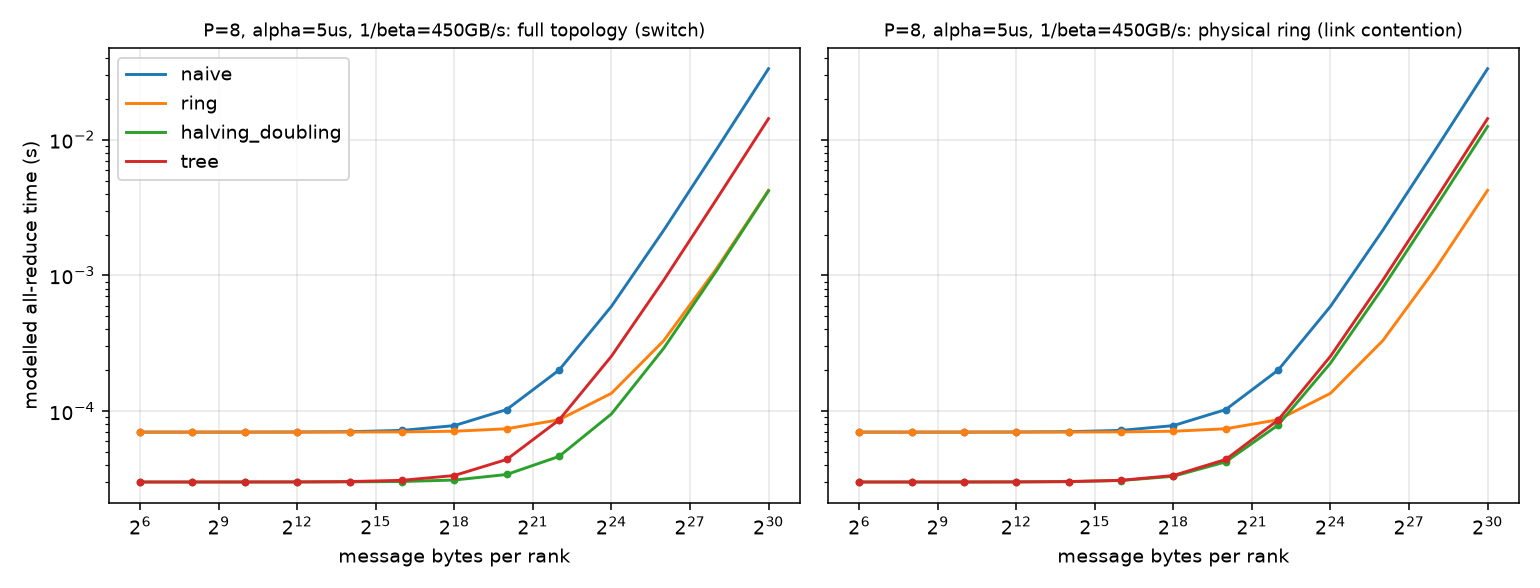
\includegraphics[width=0.82\linewidth]{allreduce_time_vs_size.png}
\caption{P=8 时四种 all-reduce 的模型时间（假设 $\alpha=5$ µs，$\beta$ 取 H100 NVLink 450 GB/s）。小消息时步数少的算法快，大消息时字节少的算法快。}
\label{fig:ar}
\end{figure}
\Cref{fig:ar} 是 \texttt{collectives.py} 的输出。模拟器逐 rank 搬运数组并统计字节，算出的时间与闭式公式一致到 $10^{-12}$。
小消息由步数决定：1 KB 时 ring 要 70.0 µs，halving-doubling 与二项树只要 30.0 µs，因为 ring 要走 $2(P-1)=14$ 步，后两者只要 $2\log_2 8 = 6$ 步。
大消息由字节决定：1 GB 时 ring 4.25 ms，halving-doubling 4.21 ms（交换机拓扑）。但换到物理环上，halving-doubling 的远距离配对会争用链路，时间升到 12.56 ms。
ring 反超树的交叉点约在 4.27 MB。所以 NCCL 同时实现 ring 与 tree、按消息大小选择，并不是冗余。

模拟器里的 $\alpha$ 和 $\beta$ 是假设的。真实实现能不能用同一个公式描述？我们在本机上跑了 gloo：

\begin{figure}[H]\centering
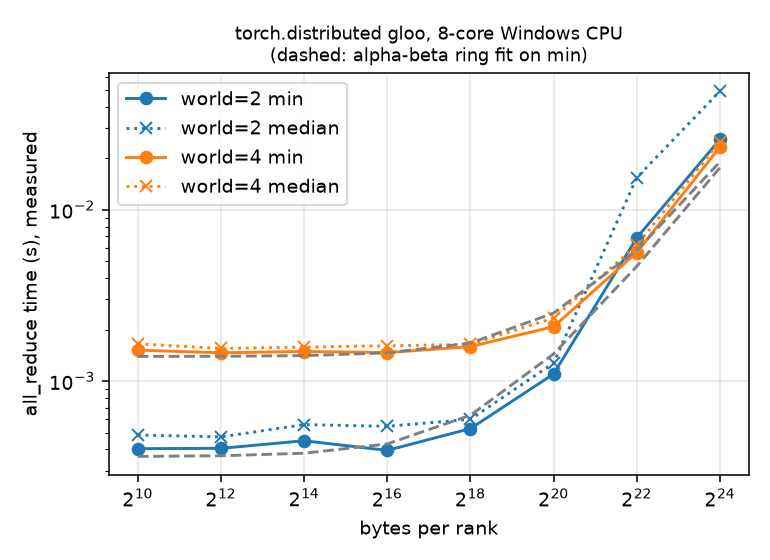
\includegraphics[width=0.7\linewidth]{gloo_allreduce.png}
\caption{本机 CPU gloo all-reduce 实测（20 次取最小）。}
\label{fig:gloo}
\end{figure}
如 \cref{fig:gloo} 所示，world=2 时 1 KB 要 0.40 ms，16 MB 要 25.8 ms。按 ring 公式拟合，得到 $\alpha\approx181$ µs、等效带宽 0.97 GB/s（world=4 时为 232 µs、1.42 GB/s）。
这个实验只说明“同一个公式能拟合真实实现”。它的数值比 NVLink 慢两到三个数量级，不能外推到 GPU 集群。

\subsection{CPU：ZeRO、流水线与重计算模型}
接下来是三种节省显存或提高利用率的方法在 CPU 模拟里的理想表现。它们给出的数字，就是后面 GPU 实测要对照的基准。

\begin{figure}[H]\centering
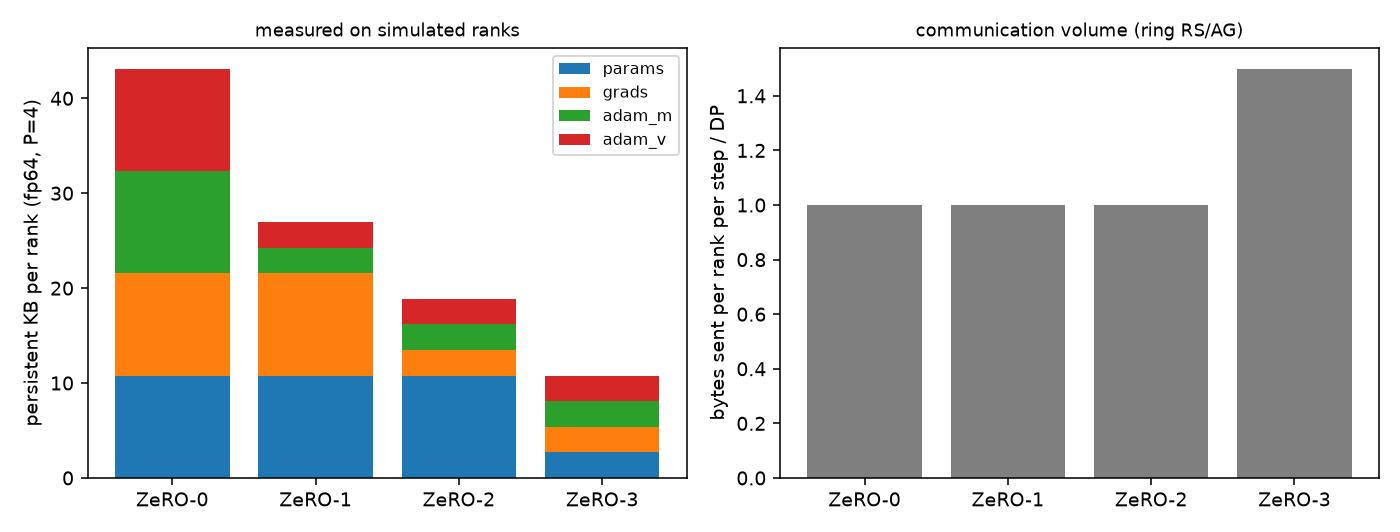
\includegraphics[width=0.85\linewidth]{zero_memory_comm.png}
\caption{ZeRO stage 0--3：左为 P=4 模拟的每 rank 常驻字节与通信量，右为论文规模（$\Psi=7.5$B、$N_d=64$）下 \texttt{mlsys\_calc} 的值。}
\label{fig:zerocpu}
\end{figure}
ZeRO 的思路是：数据并行时每张卡都存一整份优化器状态、梯度和参数，这是冗余的，可以分片存。
\Cref{fig:zerocpu} 中，fp64 模拟里四个 stage 与单进程训练的最大差为 $2.9\times10^{-16}$，说明分片不改变结果。
每 rank 常驻字节依次为 43,136 / 26,960 / 18,872 / 10,784，相对 DP 是 1 / 0.625 / 0.4375 / 0.25，与 $(1)$、$(2+2/P)/4$、$(1+3/P)/4$、$1/P$ 吻合。代价是 ZeRO-3 的通信量为 DP 的 1.5 倍。
换到论文的混合精度设置、$\Psi=7.5$B、$N_d=64$，得到 120 / 31.4 / 16.6 / 1.88 GB，与 ZeRO 论文图 1 一致。

流水线并行把模型按层切给多张卡，每张卡只算自己那几层。问题是卡与卡之间有依赖，总有一些卡在等，这段空闲叫气泡。
下面两张图是离散事件模拟的结果：

\begin{figure}[H]\centering
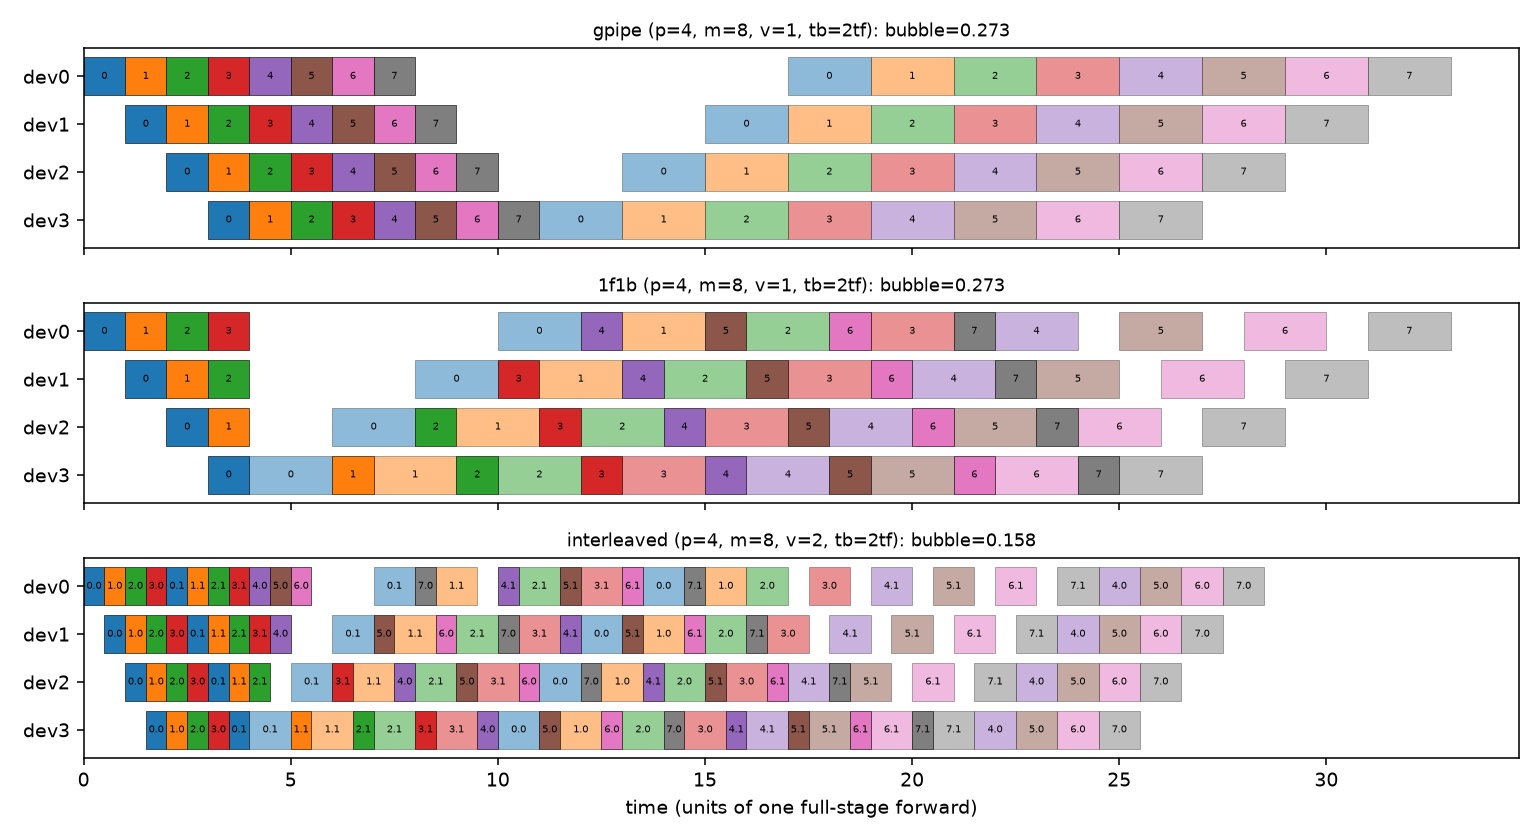
\includegraphics[width=0.9\linewidth]{pipeline_gantt.png}
\caption{离散事件模拟的 GPipe / 1F1B / 交错调度（p=4, m=8，$t_b=2t_f$）。空白处就是气泡。}
\label{fig:ganttcpu}
\end{figure}
\begin{figure}[H]\centering
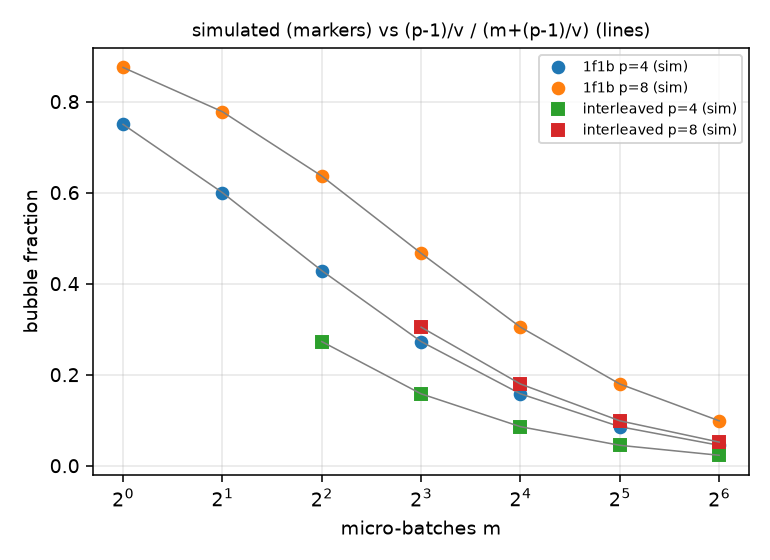
\includegraphics[width=0.7\linewidth]{pipeline_bubble.png}
\caption{模拟气泡随 micro-batch 数 $m$ 的变化，与公式 $(p-1)/(m+p-1)$ 对照。}
\label{fig:bubblecpu}
\end{figure}
从 \cref{fig:ganttcpu,fig:bubblecpu} 可以看到，算子时长均匀时，GPipe 与 1F1B 的气泡完全相同（p=4, m=8 时都是 0.273）。
1F1B 改变的只是显存：设备 0 的在途激活从 $m=8$ 份降到 $p=4$ 份。交错调度（$v=2$）把气泡降到 0.158，但设备 0 的在途激活变成 5.5，比 1F1B 还多。

重计算的思路是前向时少存一些激活，反向需要时再算一遍。问题在于存哪些、重算哪些：

\begin{figure}[H]\centering
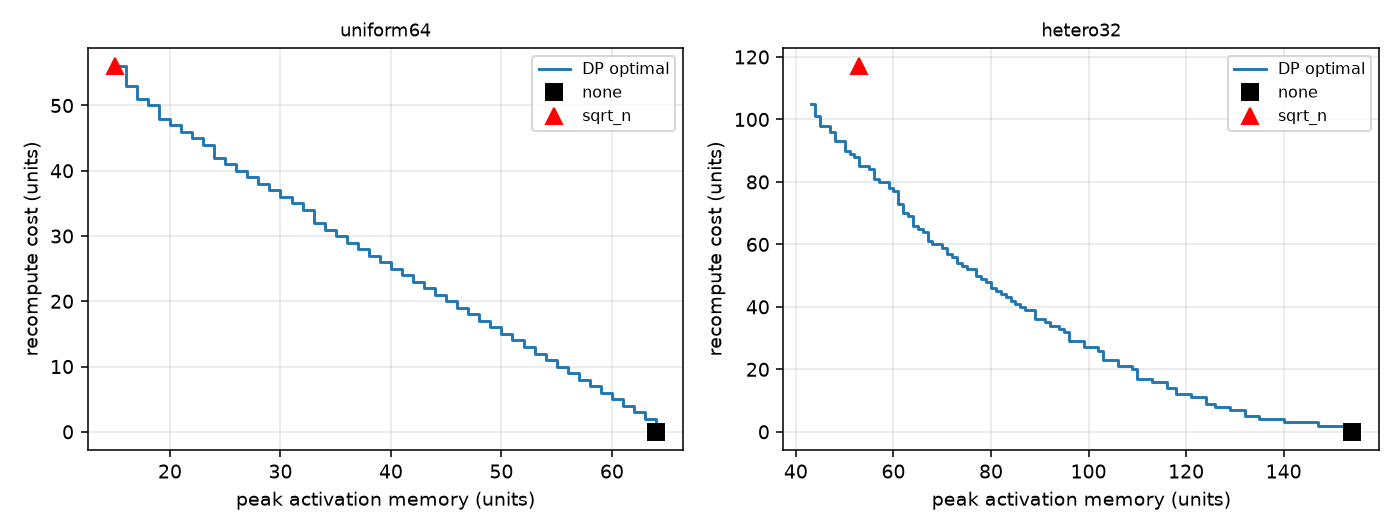
\includegraphics[width=0.75\linewidth]{ckpt_frontier.png}
\caption{重计算的显存-重算 Pareto 前沿：均匀 64 层链与异构 32 层链。}
\label{fig:ckptcpu}
\end{figure}
\Cref{fig:ckptcpu} 中，均匀的 64 层链上，$\sqrt n$ 分段（每 8 层一段）的峰值为 15、重算为 56，已经落在 DP 求出的前沿上。
层的代价不均匀时就不一样了：异构链上同样的预算 53，$\sqrt n$ 要重算 117，DP 只要 85，少 27\%。
CPU 上用 torch 跑 16 层小 MLP，时间比是 1.34--1.73，远高于理论的 4/3。原因是 Python 钩子和小算子的开销，这正是需要到 GPU 上实测的地方。

%--------------------------------------------------------------------------
\subsection{GPU A1：训练显存逐组件核算}\label{sec:mem}
估算训练显存时，最常听到的经验法则是“Adam 混合精度每参数 16 字节”。这一节把显存拆成权重、梯度、优化器状态和激活四块分别测量，看这条规则在哪些方案下成立，以及它漏掉了什么。

\begin{table}[H]\centering\scriptsize
\caption{训练显存逐组件实测（\texttt{memory.jsonl}；GB=$10^9$ 字节；B/p = (权重+梯度+优化器)/参数数；激活模型见 \cref{sec:theory-act}）}
\label{tab:mem}
\setlength{\tabcolsep}{3pt}
\begin{tabular}{llrrrrrrrrr}
\toprule
模型 & 方案 & 权重 & 梯度 & 优化器 & B/p & 激活实测 & 激活模型 & 峰值 & tokens/s & MFU \\
\midrule
gpt2-124m & fp32 & 0.50 & 0.52 & 1.01 & 16.30 & 6.54 & 6.48 & 11.34 & 54.5k & 22.4\% \\
gpt2-124m & AMP bf16 & 0.50 & 0.51 & 1.01 & 16.19 & 4.67 & 4.61 & 9.46 & 125.0k & 51.3\% \\
gpt2-124m & 纯 bf16 & 0.26 & 0.26 & 0.52 & 8.31 & 4.09 & 4.06 & 8.17 & 131.1k & 53.8\% \\
gpt2-124m & bf16+master & 0.26 & 0.26 & 1.51 & 16.32 & 4.09 & 4.06 & 9.16 & 127.9k & 52.5\% \\
gpt2-355m & fp32 & 1.42 & 1.42 & 2.84 & 16.00 & 14.61 & 14.53 & 22.17 & 20.5k & 23.8\% \\
gpt2-355m & AMP bf16 & 1.42 & 1.42 & 2.84 & 16.00 & 9.67 & 9.60 & 17.22 & 53.0k & 61.6\% \\
gpt2-355m & 纯 bf16 & 0.71 & 0.71 & 1.42 & 8.01 & 8.14 & 8.09 & 13.56 & 56.6k & 65.6\% \\
gpt2-355m & bf16+master & 0.71 & 0.71 & 4.26 & 16.01 & 8.14 & 8.09 & 16.40 & 55.2k & 64.0\% \\
gpt2-774m & fp32 & 3.17 & 3.10 & 6.19 & 16.10 & 12.96 & 12.90 & 23.97 & 9.5k & 23.7\% \\
gpt2-774m & AMP bf16 & 3.17 & 3.10 & 6.22 & 16.14 & 9.23 & 9.16 & 20.30 & 26.3k & 65.3\% \\
gpt2-774m & 纯 bf16 & 1.58 & 1.59 & 3.16 & 8.17 & 6.90 & 6.86 & 13.28 & 28.2k & 70.2\% \\
gpt2-774m & bf16+master & 1.58 & 1.57 & 9.47 & 16.31 & 6.90 & 6.86 & 19.60 & 26.8k & 66.7\% \\
\bottomrule
\end{tabular}
\end{table}
124M/355M 用 $b=8,s=1024$，774M 用 $b=4,s=1024$。表很宽，先看三列就够了：B/p 检验 16N 规则，“激活实测”与“激活模型”两列检验我们的激活公式，MFU 列留到本节最后讨论。

\begin{figure}[H]\centering
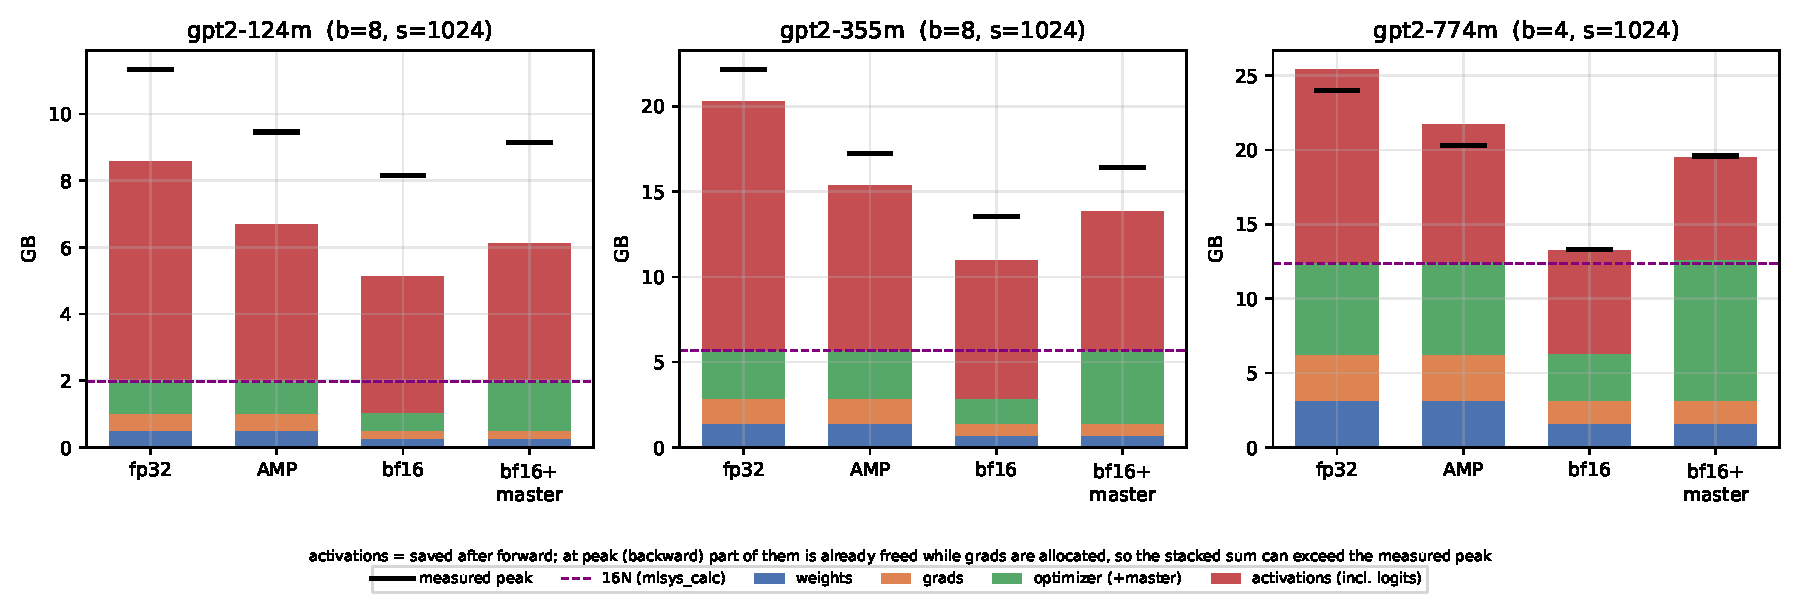
\includegraphics[width=\linewidth]{gpu_memory_breakdown.pdf}
\caption{逐组件显存堆叠图与稳态峰值（黑线），紫色虚线为 16N。三种布局的静态部分都贴着 16N，但内部的分配方式各不相同。}
\label{fig:membreak}
\end{figure}
\Cref{fig:membreak} 与 \cref{tab:mem} 说明了三件事。

第一，“16N”不是混合精度独有的。fp32（4+4+8）、PyTorch AMP（fp32 权重 4、fp32 梯度 4、m/v 共 8）和 bf16+fp32 master（2+2+12）是三种完全不同的布局，却都落在 16.00--16.32 B/参数。
差别只在 16 字节怎么分：AMP 的 16 字节里根本没有 bf16 权重，而 bf16+master 方案光优化器一项就是 12N（774M 上为 9.47 GB）。
超出 16 的那 0.0--0.3 字节，来自 CUDA 缓存分配器按 512 B 粒度取整、LayerNorm 和 bias 这类小张量，以及 fused AdamW 的 step 计数张量。

第二，纯 bf16 只要 8.01--8.31 B/参数，但它把 Adam 的 m 和 v 也放在 bf16 里。bf16 的尾数只有 7 位，长时间训练时，很小的更新会被舍入“吞掉”（见 \cref{sec:caveat}）。这是工业界仍然保留 fp32 master 的原因。

第三，真正的大头是激活。在这些 batch 下，激活是静态状态的 1.5--5.7 倍。AMP 比 fp32 省激活（355M 上 9.67 vs 14.61 GB），但不省静态显存。

\begin{figure}[H]\centering
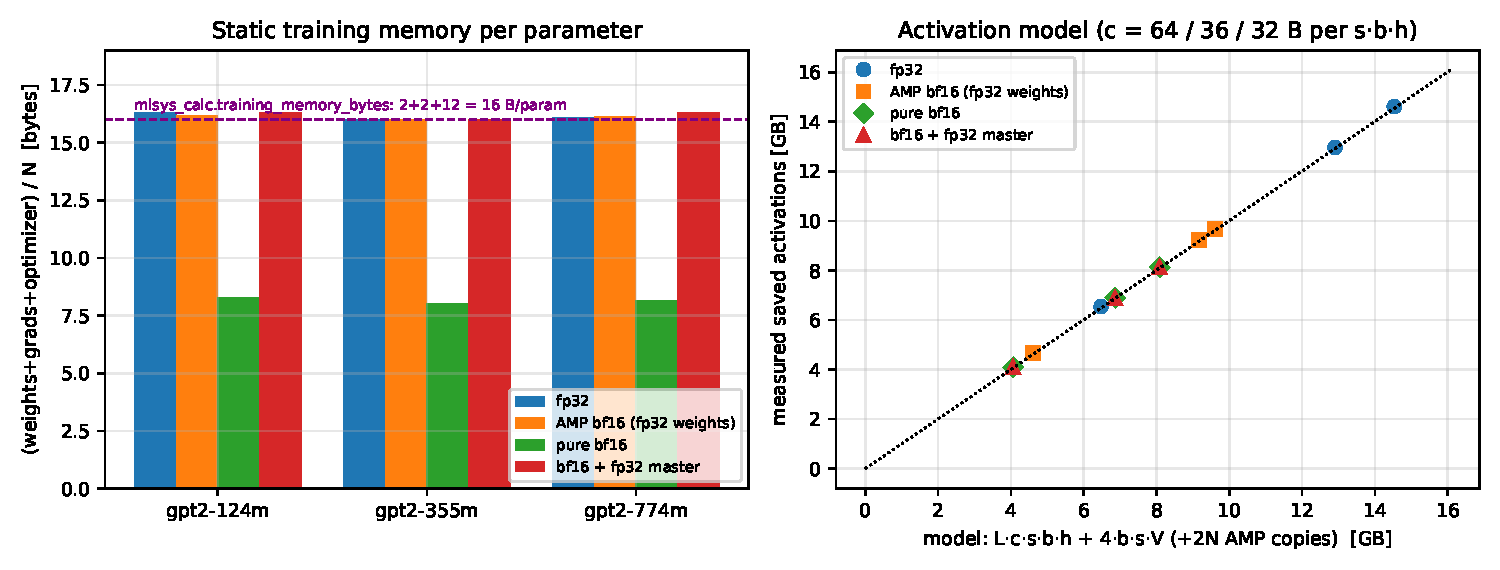
\includegraphics[width=\linewidth]{gpu_bytes_per_param.pdf}
\caption{左：静态显存/参数，与 \texttt{mlsys\_calc} 的 16 B/参数对照；右：激活模型 vs 实测（12 个配置），点几乎都落在对角线上。}
\label{fig:bpp}
\end{figure}
激活既然是大头，就值得建一个准确的模型。\Cref{fig:bpp} 右图把 \cref{sec:theory-act} 里逐张量数出来的模型和实测放在一起。
这个模型是：每层 $c\cdot s b h$ 字节，$c=64/36/32$；加上 cross-entropy 保存的 fp32 log-softmax 输出 $4bsV$；AMP 再加上 autocast 为反向保存的 bf16 权重副本，约 $2N$。
12 个配置的“实测/模型”比为 1.004--1.013。剩下约 1\% 的残差来自 embedding 输出、位置索引与 loss 标量等没有计入的小张量。

\begin{figure}[H]\centering
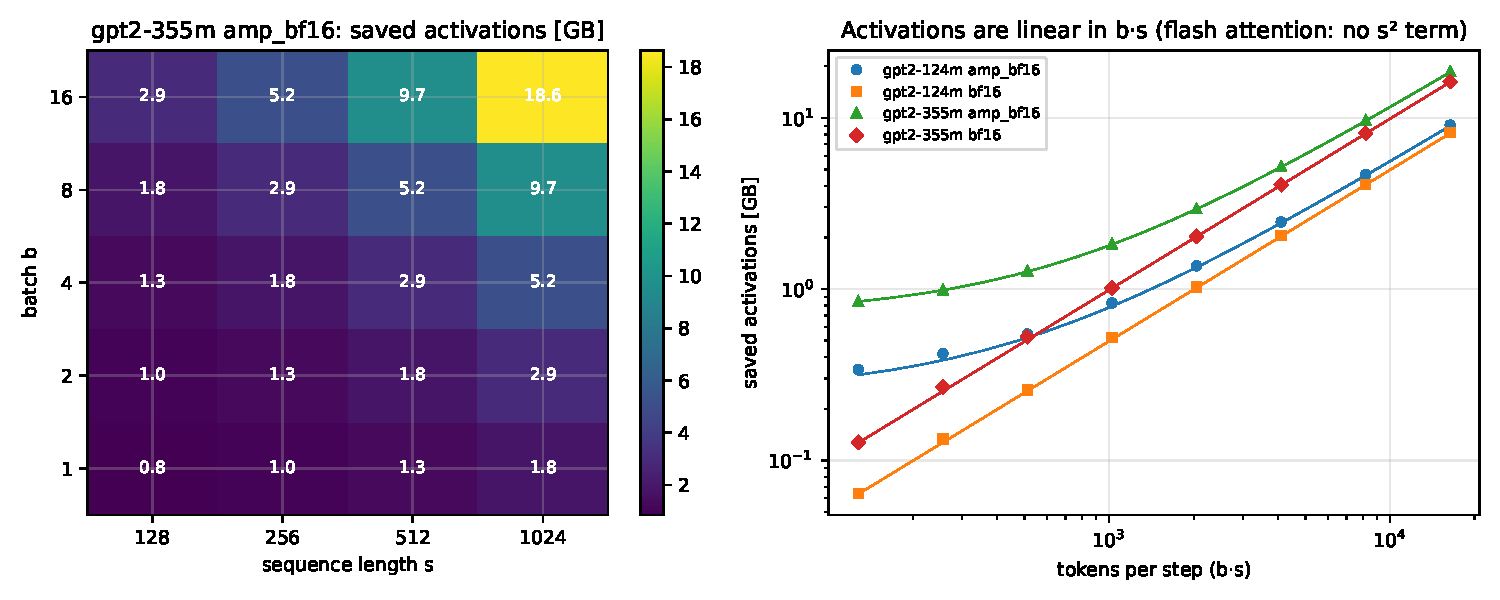
\includegraphics[width=\linewidth]{gpu_activation_sweep.pdf}
\caption{左：355M AMP 的激活随 $b\times s$ 的热力图；右：对数坐标下激活与 $b\cdot s$ 成正比（线为模型）。}
\label{fig:actsweep}
\end{figure}
模型里没有 $s^2$ 项，这一点需要单独验证，因为普通 attention 会保存 $s\times s$ 的注意力矩阵。\Cref{fig:actsweep} 显示激活对 $b\cdot s$ 严格线性：flash attention~\cite{dao2022} 确实不保存注意力矩阵。
线性拟合的斜率是 124M AMP 536,843 B/token（模型 532,804），355M AMP 1,093,862 B/token（模型 1,085,764）。
截距 272 MB / 709 MB 对应 AMP 的 bf16 权重副本（模型为 247 MB / 707 MB）；纯 bf16 没有这份副本，截距只有 4--6 MB，正好印证了“截距就是 autocast 的权重缓存”。
还有一个容易忽略的细节：每 token 的激活里，logits 项 $4V=201{,}028$ 字节占了 124M 的 38\%。词表大、模型小时，loss 那一层就是激活的大头，这也是 Megatron 和 Liger 等实现“分块 cross-entropy”的动机。

\begin{figure}[H]\centering
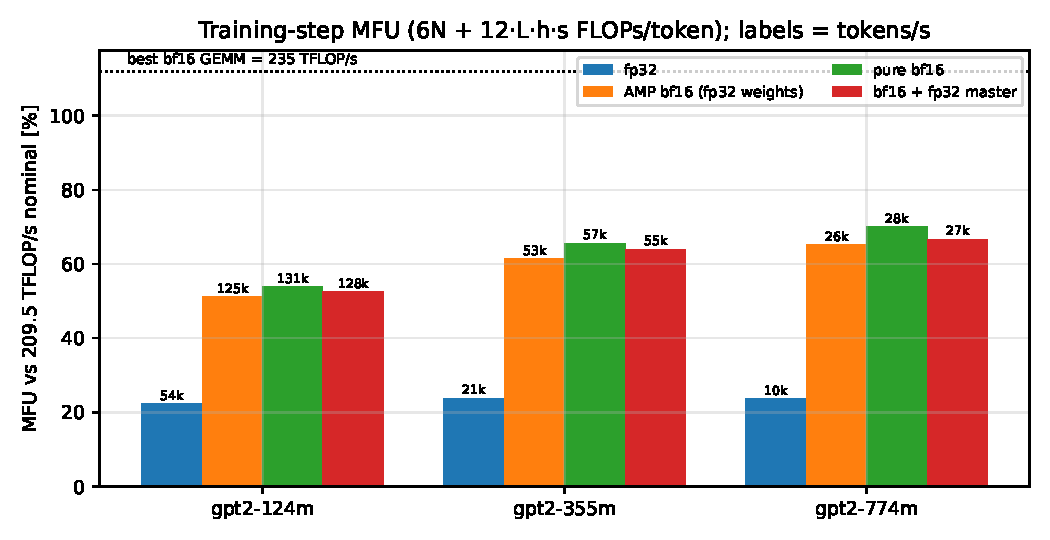
\includegraphics[width=0.8\linewidth]{gpu_mfu.pdf}
\caption{训练步 MFU（相对 209.5 TFLOP/s），柱上数字为 tokens/s；虚线为实测最佳 bf16 GEMM。}
\label{fig:mfu}
\end{figure}
最后看速度。\Cref{fig:mfu} 中，bf16 类方案的 MFU 随模型变大而升高：124M 为 51--54\%，355M 为 62--66\%，774M 为 65--70\%。
原因是隐藏维 $d$ 越大，GEMM 越接近峰值，LayerNorm、GELU 这类访存型算子的占比也越小。fp32 只有 22--24\%，因为它不走 bf16 tensor core，在 TF32 关闭时用的是 fp32 FMA。
实测 8192$^3$ 的 bf16 GEMM 达到 234.7 TFLOP/s，\emph{高于}名义的 209.5。GeForce Blackwell 上 fp32 累加并没有像上一代那样减半，
所以如果以实测 GEMM 为分母，774M 纯 bf16 的 MFU 是 $70.2\%\times209.5/234.7=62.7\%$。
bf16+master 比纯 bf16 慢约 5\%，多出来的正是每步 12N 字节的主权重读写和 fp32 梯度转换。

\begin{findingbox}[：显存核算]
16N 规则在三种布局下都成立（实测 16.00--16.32 B/参数），纯 bf16 为 8 B/参数；在 GPT-2 规模上，决定能否放下的是激活，而不是参数。
\end{findingbox}

%--------------------------------------------------------------------------
\subsection{GPU A2：激活重计算}\label{sec:recompute}
上一节说明激活才是显存大头。重计算用时间换显存，教科书给出的代价是“多 1/3 的时间”。这一节回答三个问题：真实的代价是多少，省下的显存能不能用逐张量模型解释，以及省下的显存能否换来更高的吞吐。

实验在 774M、AMP、$b=8$、$s=1024$ 上进行，对五种策略各测一次显存与步时间（\texttt{recompute.jsonl}；使用 \texttt{expandable\_segments} 分配器）。
然后对其中四种策略，在 $\{4,8,12,16,20,24,32,\dots\}$ 的阶梯上找最大可放的 batch，遇到第一次 OOM 就停。

\begin{figure}[H]\centering
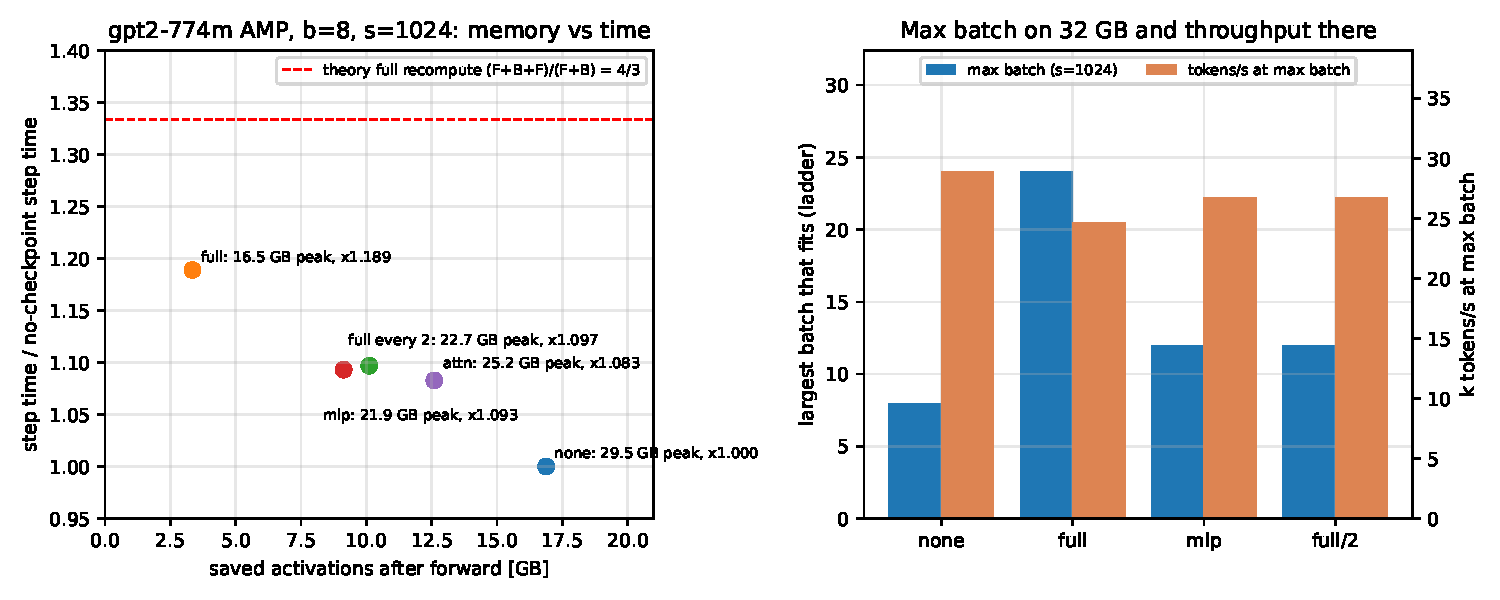
\includegraphics[width=\linewidth]{gpu_recompute.pdf}
\caption{左：前向后保存的激活 vs 步时间（均相对不 checkpoint）；越靠左下越划算。右：32 GB 上的最大 batch，以及该 batch 下的吞吐。}
\label{fig:recompute}
\end{figure}

\begin{table}[H]\centering\small
\caption{重计算的显存与时间（774M，AMP，$b=8$，$s=1024$，\texttt{recompute.jsonl}）}
\label{tab:recompute}
\begin{tabular}{lrrrrr}
\toprule
策略 & 保存激活 (GB) & 相对 & 峰值总显存 (GB) & 步时间 (ms) & 时间比 \\
\midrule
不 checkpoint & 16.880 & 1.000 & 29.47 & 282.6 & 1.000 \\
每块全量 & 3.348 & 0.198 & 16.54 & 336.1 & 1.189 \\
隔块全量（every 2） & 10.110 & 0.599 & 22.71 & 310.0 & 1.097 \\
只 MLP & 9.131 & 0.541 & 21.85 & 309.0 & 1.093 \\
只 attention & 12.599 & 0.746 & 25.20 & 306.0 & 1.083 \\
\bottomrule
\end{tabular}
\end{table}

\paragraph{显存与逐张量模型逐项吻合。} 先看显存。用 \cref{sec:theory-act} 的计数（AMP 下每层 $c=36$ 字节/$sbh$，$L\cdot sbh = 36\times8\times1024\times1280 = 3.775\times10^8$），可以逐项解释表中每一行：
\begin{itemize}
\item 不 checkpoint：$36\cdot L\,sbh + 4bsV + 2N = 13.59 + 1.647 + 1.548 = 16.785$ GB，实测 16.880 GB（比值 1.006）。
\item 只 MLP：省掉 MLP 内部的 $2+8+8=18$ 字节/$sbh$（6.795 GB），再加上 autocast 为 \texttt{fc}/\texttt{fc2} 保存的 bf16 权重副本 $8h^2\cdot2\cdot L = 0.944$ GB，
合计 7.739 GB；实测节省 $16.880-9.131=7.749$ GB。
\item 只 attention：checkpoint 的输入（fp32 残差，4 字节）仍要保存，所以只省 LN 输出 2、QKV 6、attention 输出 2，共 10 字节（3.775 GB），再加 \texttt{qkv}/\texttt{proj} 的权重副本 0.472 GB，
合计 4.247 GB；实测节省 4.281 GB。
\item 每块全量：每层只剩块输入 $4sbh$（1.510 GB），加上 $4bsV$（1.647 GB），共 3.157 GB；实测 3.348 GB。多出的 0.19 GB 恰好是最后一层 LN 的 fp32 输入（42 MB）、
它的 bf16 输出（21 MB）与 LM head 的 bf16 权重副本（$Vh\cdot2=129$ MB），这些都在 checkpoint 区域之外。
\end{itemize}
其中“只 MLP”的节省量与模型只差 0.1\%。从这笔账里还能看出，“只 MLP”是性价比最高的选择性方案：每层 36 字节里有一半在 MLP，因为 GELU 的输入和输出都是 $4h$ 宽。

\paragraph{时间远低于 4/3。} 再看时间。每块全量重计算只慢了 18.9\%，而不是理论上的 33.3\%。
$4/3$ 的推导假设整步只有块的前向与反向，并且 $B=2F$；实测的时间比说明，“块前向”只占整步的 18.9\%。
差额来自三类不会被重算的工作。一是 LM head 与 cross-entropy：$V=50257$ 时，LM head 约占前向 FLOPs 的 8\%。二是 fused AdamW，它要读写 fp32 参数、梯度和两个矩，约 21.7 GB 访存。
三是反向里比 $2F$ 更贵的部分：flash attention 的反向本身就要重算注意力分数，AMP 下还有梯度的 dtype 转换。
选择性方案的时间比为 1.083--1.097，与它们重算的 FLOPs 比例同序。MLP 占块 FLOPs 约 2/3，重算它却只多花 9.3\%，因为重算的是 GEMM，也就是整步里效率最高的部分。

\paragraph{最大 batch 与吞吐。} 最后看省下的显存能不能换来吞吐。32 GB 上，不 checkpoint 最多放 $b=8$，28.9k tokens/s，MFU 71.8\%。
每块全量重算可以放 $b=24$（3 倍），但吞吐降到 24.7k tokens/s（MFU 61.4\%）；只 MLP 与隔块全量都能放 $b=12$，约 26.7--26.8k tokens/s。
原因是 $b=8$ 时 GPU 已经饱和（MFU 72\%），更大的 batch 不再提高效率，重计算的开销\emph{没有}被吞吐收益抵消。
重计算的价值因此不在提速，而在于让原本放不下的配置变得可行：更长的序列、更大的模型，或者想要更大的全局 batch 又不想用梯度累积。

\begin{findingbox}[：重计算]
全量重计算把激活压到 19.8\%、最大 batch 提高 3 倍，时间只多 18.9\%，低于理论的 33\%，因为 LM head、优化器和更贵的反向都不被重算。
GPU 已经饱和时，重计算不会因为 batch 变大而“回本”。
\end{findingbox}

%--------------------------------------------------------------------------
\subsection{GPU A3：ZeRO 分片的每 rank 显存与通信参数}\label{sec:zero}
ZeRO 的显存公式在 CPU 模拟里已经对上了，但那是几万字节的玩具。这一节有两个目标：在真实的 774M 模型上确认公式，然后测出能代入通信模型的带宽，估算多卡上的通信代价。

\begin{figure}[H]\centering
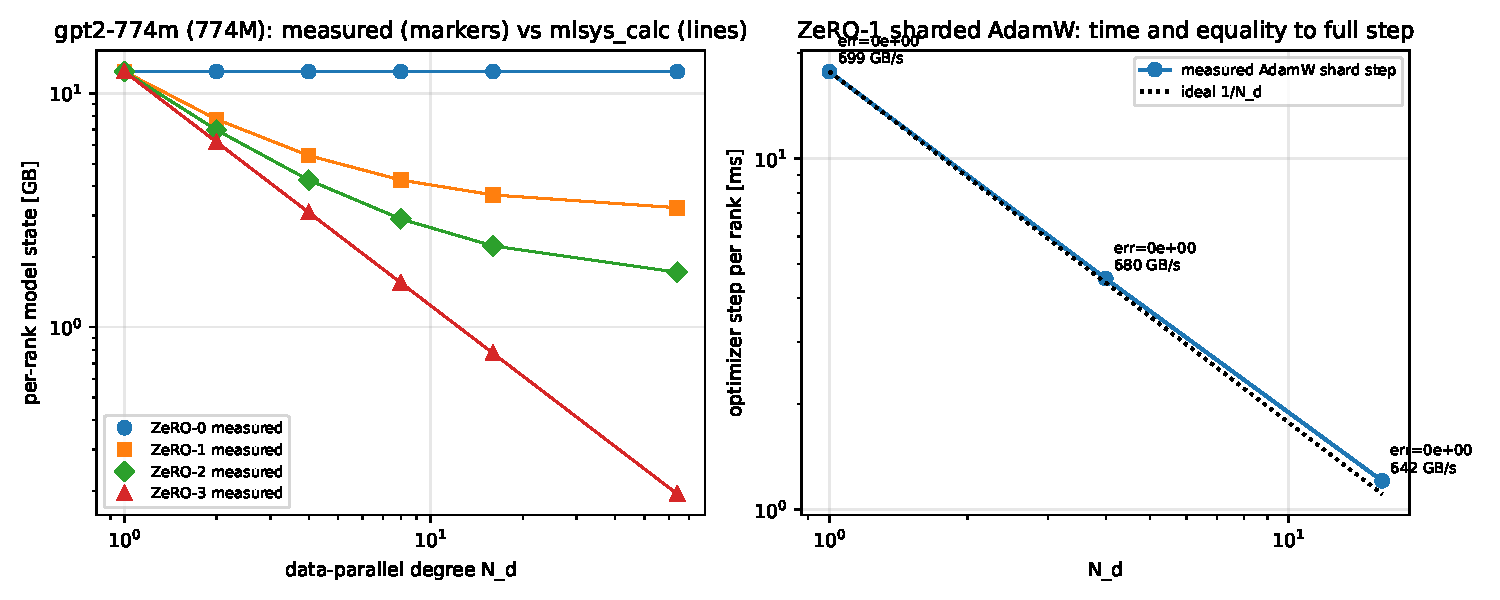
\includegraphics[width=\linewidth]{gpu_zero.pdf}
\caption{左：774M 模型的 rank 0 在 ZeRO-0..3 下真实分配的状态显存（点）与 \texttt{mlsys\_calc}（线）；右：分片 AdamW 每 rank 的步时间与等价性。}
\label{fig:zero}
\end{figure}
\begin{table}[H]\centering\small
\caption{rank 0 常驻模型状态（GB，\texttt{zero.jsonl}；$N$ = 774,030,080，bf16 权重/梯度 + fp32 master/m/v）}
\label{tab:zero}
\begin{tabular}{rrrrr}
\toprule
$N_d$ & ZeRO-0 & ZeRO-1 & ZeRO-2 & ZeRO-3 \\
\midrule
1 & 12.384 & 12.384 & 12.384 & 12.384 \\
8 & 12.384 & 4.260（模型 4.257） & 2.905（2.903） & 1.548（1.548） \\
64 & 12.384 & 3.241（3.241） & 1.718（1.717） & 0.194（0.194） \\
\bottomrule
\end{tabular}
\end{table}
\Cref{fig:zero} 左与 \cref{tab:zero} 中，24 个 $(N_d,\text{stage})$ 组合的实测值与 \texttt{mlsys\_calc.\allowbreak{}training\_\allowbreak{}memory\_\allowbreak{}bytes(N, dp, zero)} 的最大相对误差为 0.099\%，来自补齐到 $N_d$ 倍数的 padding 和分配器取整。
这个实验的意义不在于“分配多少就是多少”，而在于把公式落到真实模型的扁平化参数上，看清每个 stage 实际省了多少。
ZeRO-1 在 $N_d=8$ 时把 12.38 GB 压到 4.26 GB（$-66\%$），774M 的模型状态已经能放进 8 GB 的卡；ZeRO-2 再省 1.35 GB；
只有 ZeRO-3 能让状态随 $N_d$ 线性下降（$N_d=64$ 时 0.194 GB），代价是前向和反向各多一次参数 all-gather。
$N_d$ 很大时，ZeRO-1 和 ZeRO-2 分别有 $4N$ 与 $2N$ 字节（3.10 / 1.55 GB）的下限降不下去。这就是“大模型只能用 ZeRO-3/FSDP~\cite{zhao2023}”的定量原因。

右图检验的是收敛性。对 $N_d\in\{1,4,16\}$ 逐 rank 执行两步分片 fused AdamW 并拼回，结果与整张量 AdamW \textbf{逐位相等}（max abs err = 0）。
AdamW 是逐元素算子，分片不改变任何浮点运算的顺序，所以 ZeRO-1 不会改变收敛性。
每 rank 的步时间为 17.7 / 4.55 / 1.21 ms，与 $1/N_d$ 吻合。fused AdamW 每个参数读 $p,g,m,v$、写 $p,m,v$，共 28 字节；$N_d=1$ 时对应 $28\times774\text{M}/17.7\,\text{ms}=1.22$ TB/s，约为实测拷贝带宽的 80\%。
优化器步纯粹受访存限制，所以它的时间也按 ZeRO 的分片比例下降。

显存问题解决之后，剩下的是通信。单卡上能测到哪些通信参数？

\begin{figure}[H]\centering
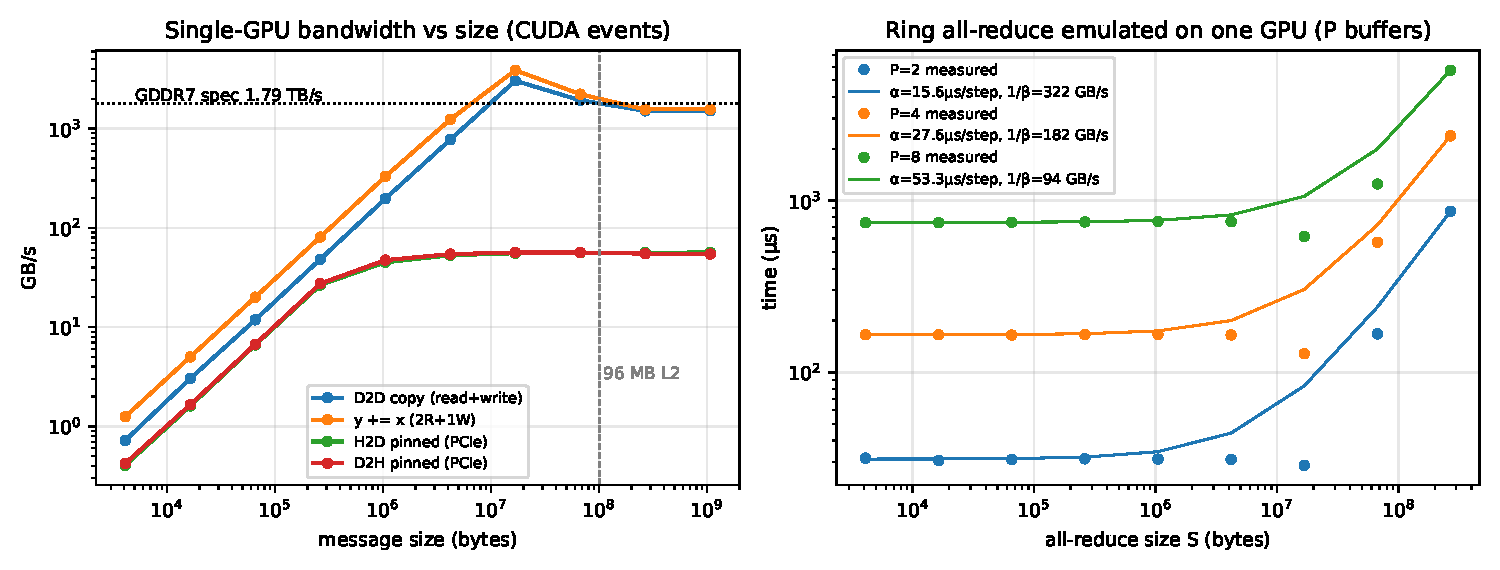
\includegraphics[width=\linewidth]{gpu_bandwidth_ring.pdf}
\caption{左：单卡上四类“链路”的带宽随消息大小的变化；右：单卡 ring all-reduce 仿真（$P$ 个缓冲区）与 $\alpha$-$\beta$ 拟合。}
\label{fig:bw}
\end{figure}
\Cref{fig:bw} 左图中，D2D 拷贝在 16 MB 时达到 3.04 TB/s（读加写计），这是数据驻留在 96 MB L2 里造成的假象；超过 L2 后稳定在 1.52 TB/s（1 GiB），为 GDDR7 名义 1.79 TB/s 的 85\%。
pinned H2D/D2H 稳定在 56.5 / 54.5 GB/s，是 PCIe 5.0 x16 理论 64 GB/s 的 88\%。
所有曲线在 $\le 64$ KB 时都是一条斜率为 1 的直线，即时间固定在约 10 µs，这就是启动和同步的开销 $\alpha$。
右图中，单卡 ring 在 $\le 4$ MB 时完全平坦：P=8 时是 743 µs，等于 $2(P-1)\cdot P=112$ 次启动乘以 6.6 µs。拟合出每步的 $\alpha$ 为 15.6 / 27.6 / 53.3 µs（P=2/4/8）。
大消息一端的“总线带宽”322 / 182 / 94 GB/s 只反映 $P$ 份缓冲共用一块 HBM，不代表任何互连。
数值正确性方面，它与 \texttt{torch.stack(...).sum(0)} 的最大差 $\le 2.9\times10^{-6}$，来自 fp32 求和顺序的不同。

单卡测不到互连，但 PCIe 带宽是真实的。把它代回 ZeRO 的通信量，就能估算一台没有 NVLink 的多卡 5090 机器：

\begin{figure}[H]\centering
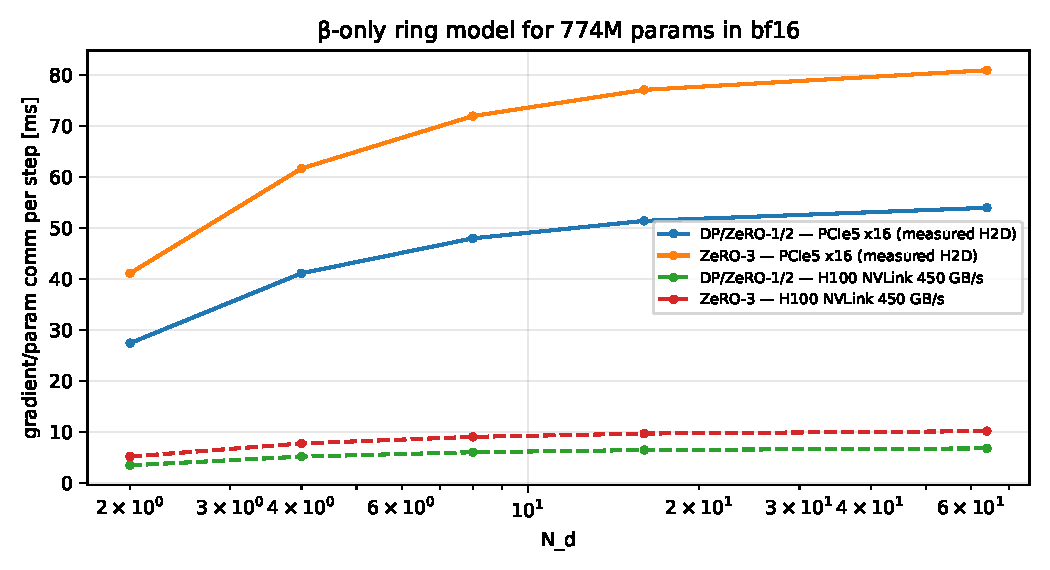
\includegraphics[width=0.8\linewidth]{gpu_zero_comm.pdf}
\caption{用实测 PCIe 带宽与 H100 NVLink 参数估算的 ZeRO 每步通信时间（774M，bf16，只计 $\beta$ 项）。}
\label{fig:zerocomm}
\end{figure}
\Cref{fig:zerocomm} 中，DP、ZeRO-1 和 ZeRO-2 每步通信 $2\Psi$（RS+AG），ZeRO-3 为 $3\Psi$。在 $N_d=8$ 的 PCIe 5090 机器上，774M 的 DP 每步要 47.97 ms，ZeRO-3 要 71.96 ms；H100 NVLink 上 DP 只需 6.02 ms。
单卡计算一步约 145 ms（$b=4$），所以 PCIe 上 DP 的通信/计算比约 0.33，ZeRO-3 约 0.50。
这部分通信能否靠重叠藏起来，取决于反向里梯度分桶的粒度，以及 PCIe 是否同时被 H2D 数据加载占用。

\begin{findingbox}[：ZeRO]
每 rank 状态与 $(2+2+12)N$ 的分片公式误差 $<0.1\%$，分片 AdamW 与整张量逐位相等。真正决定多卡 5090 训练的是 PCIe 的 56.5 GB/s，它让 DP 通信达到计算时间的 1/3。
\end{findingbox}

%--------------------------------------------------------------------------
\subsection{GPU A4：真实 kernel 的 GPipe 与 1F1B}\label{sec:pipeline}
CPU 模拟假设每一级的算子时长完全相同。真实模型里，第一级要做 embedding，最后一级要做 LM head 和 loss，各级并不均衡。
这一节用真实 kernel 的时长重放流水线，检验两个论文命题：1F1B 的在途激活不超过 $p$，以及气泡等于 $(p-1)/(m+p-1)$。

\begin{figure}[H]\centering
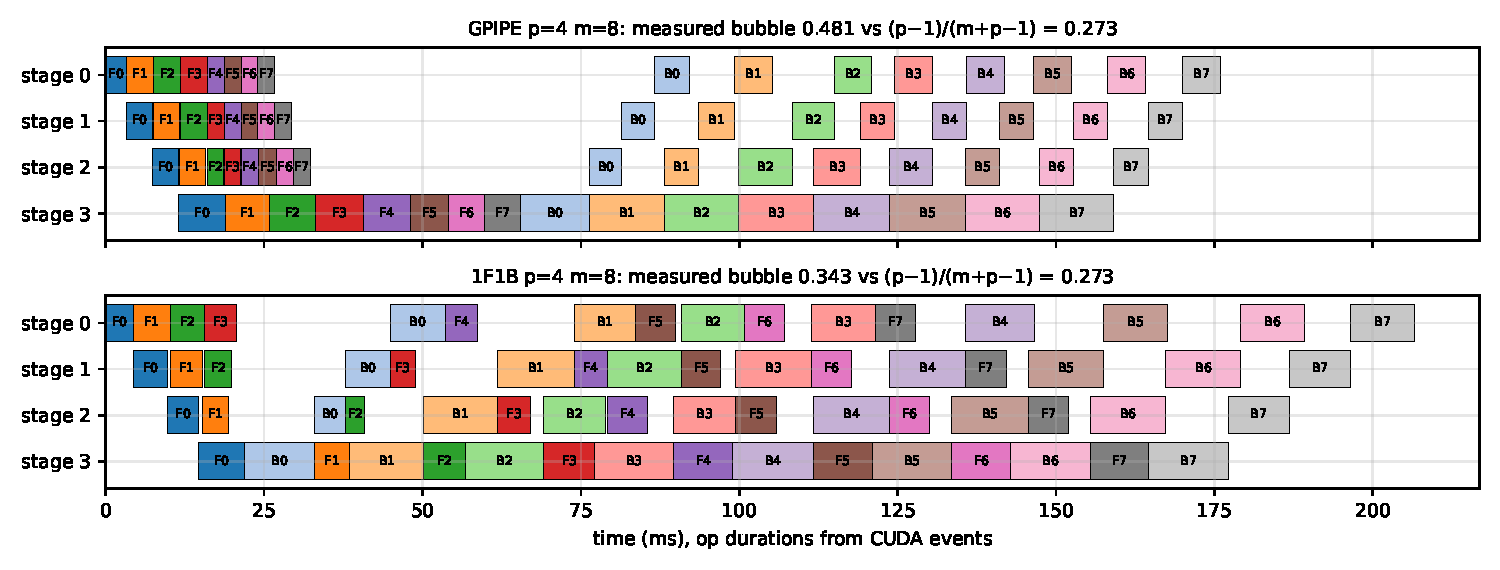
\includegraphics[width=\linewidth]{gpu_pipeline_gantt.pdf}
\caption{GPT-2 355M 切成 4 级（每级 6 块；stage 0 含 embedding，stage 3 含 LM head + loss），micro-batch 为 $4\times512$，$m=8$。
每个色块的长度是该算子的 CUDA event 实测时长，起止时刻按依赖关系重放。最后一级的色块明显更长。}
\label{fig:gantt}
\end{figure}
\begin{table}[H]\centering\small
\caption{流水线实测（\texttt{pipeline.jsonl}；p=4；“不均衡模型”= $(m-1)T_{\max}+\sum_d T_d$，$T_d=t_f^d+t_b^d$ 取该次运行各级的中位数）}
\label{tab:pipe}
\setlength{\tabcolsep}{4pt}
\begin{tabular}{lrrrrrrr}
\toprule
调度 & $m$ & 气泡实测 & $(p-1)/(m+p-1)$ & 不均衡模型 & makespan (ms) & 峰值显存 (GB) & 每级在途 mb \\
\midrule
GPipe & 1 & 0.750 & 0.750 & 0.750 & 45.5 & 3.77 & [1,1,1,1] \\
GPipe & 4 & 0.521 & 0.429 & 0.497 & 113.4 & 12.61 & [4,4,4,4] \\
GPipe & 8 & 0.481 & 0.273 & 0.502 & 175.9 & 24.40 & [8,8,8,8] \\
GPipe & 16 & \multicolumn{6}{c}{OOM（32 GB）} \\
1F1B & 4 & 0.492 & 0.429 & 0.481 & 117.5 & 7.64 & [4,3,2,1] \\
1F1B & 8 & 0.343 & 0.273 & 0.354 & 206.6 & 7.64 & [4,3,2,1] \\
1F1B & 16 & 0.245 & 0.158 & 0.254 & 389.9 & 7.64 & [4,3,2,1] \\
1F1B & 32 & 0.233 & 0.086 & 0.203 & 723.9 & 7.64 & [4,3,2,1] \\
\bottomrule
\end{tabular}
\end{table}

\Cref{fig:gantt,tab:pipe} 给出三条结论。

\paragraph{在途激活完全符合 1F1B 的论文命题。} 1F1B 下每级在途 micro-batch 的峰值恰好是 $[p-d] = [4,3,2,1]$，与 $m$ 无关；GPipe 下是 $[m,m,m,m]$。
单卡执行全部 4 级时的真实峰值显存也是如此：GPipe 从 3.77 GB（$m=1$）涨到 24.40 GB（$m=8$），$m=16$ 时 OOM；1F1B 在 $m\ge4$ 之后恒为 7.64 GB。
每级每个 micro-batch 的激活实测为 613 / 605 / 605 / 1124 MB。stage 3 多出的约 520 MB，正是 $4\cdot bsV = 4\times4\times512\times50257=412$ MB 的 fp32 log-softmax，再加 bf16 权重副本。

\paragraph{气泡公式只在各级均衡时成立。} 实测气泡全部高于 $(p-1)/(m+p-1)$，而且 1F1B 在 $m=32$ 时停在 0.233，而不是公式的 0.086。
原因就是各级不均衡：在 $m=32$ 的 1F1B 运行中，stage 3 的 $t_f+t_b$ 约 21.9 ms，前三级约 16.5--18.4 ms。
稳态下流水线的节拍由最慢的一级决定，makespan $\approx (m-1)T_{\max} + \sum_d T_d$，所以 $m\to\infty$ 时气泡趋向 $1-\bar T/T_{\max}$，而不是 0。
这个不均衡模型对 10 次运行的预测与实测相差 $\le0.03$（例如 GPipe $m=8$：176.3 vs 175.9 ms）。
由此可以推出，切分流水线时要把 embedding 和 LM head 单独计入代价（Megatron 的 \texttt{--decoder-first/last-pipeline-num-layers} 就是做这件事的），否则加再多 micro-batch 也压不下气泡。

\paragraph{GPipe 与 1F1B 的 makespan 相近，1F1B 并不更快。} $m=8$ 时 GPipe 是 175.9 ms，1F1B 是 206.6 ms。理论上两者相同，这里的差异来自算子时长在不同运行之间的波动（见下文）。
1F1B 的价值在显存：同样 32 GB，GPipe 最多用到 $m=8$（气泡 0.481），1F1B 可以用到 $m=32$（气泡 0.233）。
按重放口径算，两者的等效吞吐分别是 93.1k 与 90.5k tokens/s，几乎相同，原因是 1F1B 那几次运行的算子时长整体偏长。
如果用同一组算子时长，气泡从 0.481 降到 0.233，意味着吞吐提升 $(1-0.233)/(1-0.481)=1.48$ 倍。

下面两张图把气泡和显存随 $m$ 的变化，以及一步之内的显存轨迹画了出来：

\begin{figure}[H]\centering
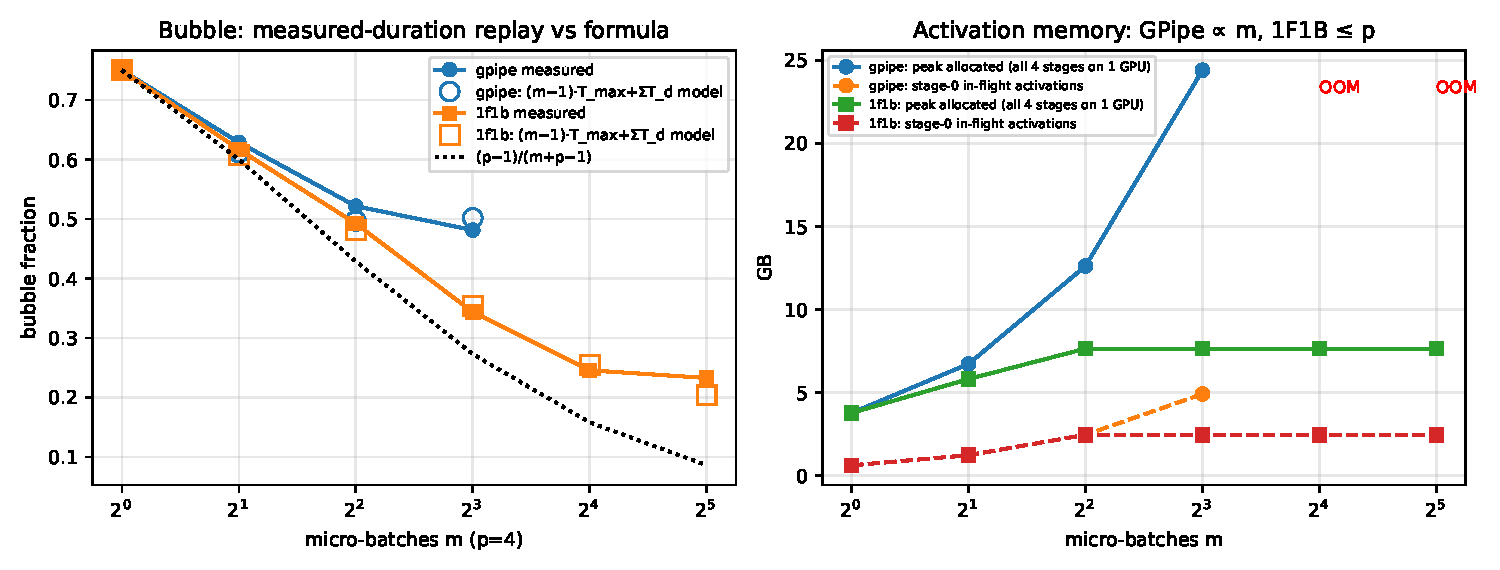
\includegraphics[width=\linewidth]{gpu_pipeline_bubble_memory.pdf}
\caption{左：气泡随 $m$ 的变化（实线为实测，空心点为不均衡模型，点线为均衡公式）；不均衡模型贴着实测，均衡公式偏低。右：峰值显存与 stage 0 的在途激活。}
\label{fig:pipebm}
\end{figure}
\begin{figure}[H]\centering
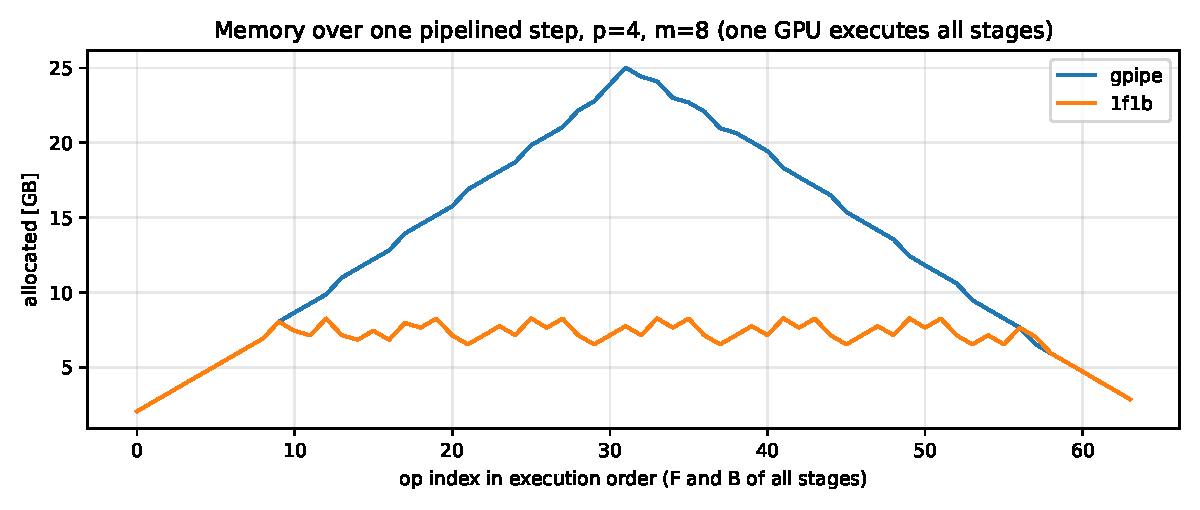
\includegraphics[width=0.8\linewidth]{gpu_pipeline_memtrace.pdf}
\caption{一次流水线步内的显存轨迹（$m=8$）：GPipe 先把 32 个前向的激活全部堆起来，1F1B 在稳态里每做一个 F 就释放一个 B。}
\label{fig:memtrace}
\end{figure}
\Cref{fig:memtrace} 直观地展示了两者显存行为的差别：GPipe 的轨迹是“先涨到顶再降下来”的三角形，1F1B 则是一段平台。

\paragraph{测量口径的局限。} 单卡无法让 4 级真正并行，所以 Gantt 图是“真实算子时长加依赖重放”，不包含 p2p 通信，也不包含多卡上算子并发时的相互干扰。
另外，同一个算子在不同运行里的时长差别明显。例如 stage 0 的前向，GPipe $m=8$ 时中位数 2.96 ms，1F1B $m=8$ 时是 5.66 ms。
这些算子只有 6 层、2048 个 token，GPU 时间约 2--3 ms，而 CPU 只有 2 个受 cgroup 配额限制的核；CPU 下发跟不上时，CUDA event 之间会混进 GPU 的空等时间。
因此本节的绝对毫秒数只作量级参考。不过每次运行内部用的是同一组时长做重放，气泡与模型的比较是自洽的。

\begin{findingbox}[：流水线]
1F1B 的在途激活实测恰为 $[4,3,2,1]$，峰值显存与 $m$ 无关（7.64 GB）。气泡公式 $(p-1)/(m+p-1)$ 假设各级均衡；LM head 让最后一级重了 20--30\%，实测气泡因此停在 0.23 附近，用 $(m-1)T_{\max}+\sum T_d$ 可以预测到 $\pm0.03$。
\end{findingbox}

%==========================================================================
\section{与理论模型的对照}

前面的实测都拿来和几条公式对照。这一节把这些公式推一遍，并说明每个实测数字是怎样代进去的。

\subsection{静态显存：16N 的三种拆法}
设参数数为 $N$。Adam 要为每个参数保存一阶矩 $m$ 和二阶矩 $v$。四种方案的静态显存分别是：
\begin{align}
\text{fp32:}\quad & 4N_{\text{w}} + 4N_{\text{g}} + 8N_{m,v} = 16N \\
\text{AMP (fp32 主权重即模型权重):}\quad & 4N + 4N + 8N = 16N \\
\text{bf16 + fp32 master（ZeRO/Megatron）:}\quad & 2N + 2N + (4+4+4)N = 16N \label{eq:16n}\\
\text{纯 bf16:}\quad & 2N + 2N + 4N = 8N
\end{align}
\texttt{mlsys\_calc.training\_memory\_bytes} 实现的是 \cref{eq:16n}，它的分项（2/2/12）只与 bf16+master 方案逐项吻合。
774M 上实测 1.58/1.57/9.47 GB，模型为 1.55/1.55/9.29 GB（$N$=774,030,080 时 $2N=1.548$ GB，$12N=9.288$ GB），1--2\% 的差异来自分配器取整与小张量。
AMP 的总量同样是 16N，只是分项为 4/4/8。所以面试里说“混合精度省一半显存”是错的：它省的是激活和带宽，不是静态状态。

\subsection{激活：逐张量计数}\label{sec:theory-act}
激活模型的做法很朴素：把反向需要保存的张量一个个数出来。对一个 pre-LN 的 GPT 块（无 dropout，使用 flash attention），以 $sbh$ 个元素为单位，需要保存的有：
LN1 输入 1，QKV 线性层的输入 1，$q,k,v$ 共 3，attention 输出 1（它同时也是输出投影的输入，因为 flash kernel 的输出缓冲布局是 $[B,T,H,D]$，
\texttt{transpose+reshape} 只是 view，不复制），LN2 输入 1，FC 输入 1，GELU 输入 4，FC2 输入（即 GELU 输出）4，共 16 个。于是每层
\begin{equation}
A_{\text{layer}} = c\cdot s b h,\qquad c=\begin{cases}16\times4=64 & \text{fp32}\\ 16\times2=32 & \text{纯 bf16}\\ 32+2\times2=36 & \text{AMP（残差流与两个 LN 输入为 fp32）}\end{cases}
\end{equation}
此外还要加上 cross-entropy 保存的 fp32 log-softmax 输出 $4bsV$（bf16 的 logits 本身不被保存），以及 AMP 为反向保存的 bf16 权重副本，约 $2N$。

这个结果可以和文献对上。Korthikanti 等~\cite{korthikanti2022} 给出 fp16 下每层 $sbh(34+5as/h)$：attention 11（QKV 输入 2、$Q,K$ 4、$V$ 2、投影输入 2、dropout 掩码 1），
MLP 19（输入 2、GELU 输入 8、GELU 输出 8、掩码 1），两个 LN 4，以及注意力分数、softmax 和 dropout 的 $5as^2b$。
去掉两个 1 字节的 dropout 掩码，再去掉 flash attention 不保存的 $s^2$ 项，正好剩下 $34-2=32$，与本文纯 bf16 的 $c=32$ 逐项对应。
这个模型并不是一次就对的。最初我们把 attention 输出和投影输入当成两个张量（共 17 个），得到 68/38/34，系统性地高估了约 6\%；是实测把它纠正成了 16 个（经过见面试专题里的 STAR 故事）。

\subsection{训练步时间与 MFU}
每 token 的训练 FLOPs 约为 $6N + 12Lhs$。774M、$s=1024$ 时，$6N=4.643\times10^9$，$12Lhs=0.566\times10^9$，合计 $5.209\times10^9$。
纯 bf16 实测 28.2k tokens/s，得到 $1.47\times10^{14}$ FLOP/s，即名义峰值的 70.2\%。
这比 Megatron 和 PaLM 报告的大模型 MFU（40--60\%）要高，因为单卡没有任何通信，而且 GPT-2 774M 的 GEMM（$h=1280$，$4h=5120$）已经足够大。

\subsection{$\alpha$-$\beta$ 模型的单卡定参}
Ring all-reduce 的时间为 $T = 2(P-1)\alpha + 2\frac{P-1}{P}S\beta$。单卡 ring 仿真里每一步有 $P$ 次 kernel 启动，小消息时的平台给出每步的 $\alpha$：
$P=2,4,8$ 时分别为 15.6、27.6、53.3 µs，折合每次启动约 6.7--7.8 µs，与 4 KB 拷贝的 10--11 µs 事件计时一致。
大消息端的“总线带宽”322/182/94 GB/s 随 $P$ 下降，因为所有“链路”共享同一块 HBM：$P$ 个 rank 同时搬运，单卡 1.52 TB/s 的 HBM 带宽被 $P$ 份分摊，再除以拷贝加法的 3 次访存。
所以单卡仿真能测出 $\alpha$（启动和同步开销）并验证算法正确（误差 $\le2.9\times10^{-6}$，来自 fp32 求和顺序），但\textbf{不能}测出互连的 $\beta$。

真正可用的 $\beta$ 来自 PCIe：pinned H2D 56.5 GB/s，D2H 54.5 GB/s（1 GiB）。代入 774M、bf16 梯度（$2N=1.548$ GB）、$N_d=8$：
\begin{equation}
T_{\text{DP}} = 2\cdot\tfrac{7}{8}\cdot\frac{1.548\,\text{GB}}{56.5\,\text{GB/s}} = 47.9\,\text{ms},\qquad
T_{\text{ZeRO-3}} = 1.5\,T_{\text{DP}} = 71.9\,\text{ms}
\end{equation}
而 774M 单步计算（$b=4,s=1024$）约 145 ms（\cref{tab:mem}，28.2k tokens/s）。也就是说，在 8 卡 PCIe 5090 上做 DP，通信约占计算的 1/3，
必须靠梯度分桶并与反向重叠才能藏住；ZeRO-3 额外的 0.5 倍通信几乎藏不住。同样的通信量在 H100 NVLink（450 GB/s）上只要 6.0 ms。

\subsection{流水线气泡：均衡与不均衡}
各级均衡时，设每级前向加反向耗时 $T$，GPipe 和 1F1B 的 makespan 都是 $(m+p-1)T$，有效工作为 $mpT$，所以气泡为 $(p-1)/(m+p-1)$（\texttt{mlsys\_calc.pipeline\_bubble}）。
不均衡时，稳态节拍取最慢一级的 $T_{\max}$。第一个 micro-batch 穿过全部各级要 $\sum_d T_d$，此后每隔 $T_{\max}$ 出来一个，于是
\begin{equation}
\text{makespan} \approx (m-1)\,T_{\max} + \sum_{d} T_d,\qquad
\text{bubble} = 1 - \frac{m\sum_d T_d}{p\left[(m-1)T_{\max}+\sum_d T_d\right]}\ \xrightarrow{m\to\infty}\ 1-\frac{\bar T}{T_{\max}}.
\end{equation}
代入 1F1B $m=32$ 的实测 $T_d$ = 16.5/18.2/18.4/21.9 ms，极限气泡为 $1-18.7/21.9=0.14$，有限 $m$ 时为 0.203，实测是 0.233。

\subsection{重计算的时间与显存}
全量重计算（每块 checkpoint）时，反向之前要把每块的前向再做一遍：$T = F + B + F$，取 $B\approx2F$ 得 $T/T_0 = 4/3$。
显存上只保留每块的输入（AMP 下残差流为 fp32，每层 $4sbh$ 字节），再加上“正在重算的那一块”的完整激活：
\begin{equation}
A_{\text{full}} \approx L\cdot 4sbh + c\cdot sbh + 4bsV,\qquad A_{\text{none}} = L\cdot c\cdot sbh + 4bsV \ (+2N).
\end{equation}
774M（$L=36$, $c=36$）时，块内激活压缩到约 $4/36=1/9$，但 logits 项 $4bsV$ 不受影响，所以全量重计算之后的激活不会降到 1/9。
选择性重计算只 checkpoint MLP 时，从每层的 $c$ 中去掉 MLP 的 $2+8+8=18$ 字节（AMP 下 FC 输入 2、GELU 输入 8、GELU 输出 8），时间代价只是一次 MLP 前向，约占块 FLOPs 的 2/3。
只 checkpoint attention 子层则只省 $2+6+2=10$ 字节，因为子层输入那 4 字节的 fp32 残差作为 checkpoint 的输入仍要保存；而 flash attention 下，注意力部分的 FLOPs 本来就小。
两种选择性方案还会省掉对应线性层的 autocast bf16 权重副本（MLP 每层 $8h^2\cdot2$ 字节，attention 每层 $4h^2\cdot2$ 字节），实测见 \cref{tab:recompute}。

\subsection{$\sqrt n$ 与 Checkmate}
Chen 2016 的 $\sqrt n$ 分段把 $n$ 层的峰值从 $O(n)$ 降到 $O(\sqrt n)$，代价是多一次前向；Checkmate 则用 MILP 在异构图上求最优解。
本 lab 的 CPU DP 在异构 32 层链上比 $\sqrt n$ 少 27\% 的重算。GPU 实验里我们只比较了“每块、隔块、子层”这几种工程上最常见的策略，它们对应 Megatron 的 \texttt{full} 与 \texttt{selective} 两档。

%==========================================================================
\section{面试专题}

\begin{iqbox}{训练一个 7B 模型，Adam 混合精度，需要多少显存？}
光静态状态就要 $16\Psi = 112$ GB，还没算激活：bf16 权重 2 字节、bf16 梯度 2 字节、fp32 的 master/m/v 共 12 字节。本文在 774M 上实测 bf16+master 为 16.31 B/参数，与公式差 2\%。
单卡 80 GB 放不下，至少要用 ZeRO-1：$N_d=8$ 时每卡 $(4+12/8)\Psi=38.5$ GB。
\par 常见的错答有两种：一是“bf16 训练，每参数 2 字节，所以 14 GB”，漏了梯度和优化器；二是“混合精度比 fp32 省一半”，其实静态状态一样是 16 字节，省的是激活和带宽。
\end{iqbox}

\begin{iqbox}{激活显存怎么估？为什么你的公式是 32 而 Megatron 论文是 34？}
逐个数出反向要保存的张量，每层 $c\cdot sbh$ 字节，再加 loss 的 $4bsV$。纯 bf16、无 dropout、用 flash attention 时，一共 16 个 $sbh$ 张量，即 32 字节。
Megatron 的 34 多了两个 dropout 掩码，$5as/h$ 那一项是不用 flash 时要保存的注意力分数。本文 12 个配置的实测/模型 = 1.004--1.013。
\par 常见的错答是忘掉 logits 项：GPT-2 124M、$V$=50257 时，它占每 token 激活的 38\%。另一个错答是以为 AMP 的激活是纯 bf16 的一半，其实残差流仍是 fp32，是 36 对 32。
\end{iqbox}

\begin{iqbox}{activation checkpointing 的时间代价是多少？}
理论上全量重计算是 $4/3$，因为多了一次前向；但 774M 实测只慢 18.9\%，因为 LM head、优化器步和比 $2F$ 更贵的反向都不会被重算。
它把激活降到 19.8\%，最大 batch 从 8 提到 24。只重算 MLP 时慢 9.3\%，省 46\% 的激活。
要注意，GPU 已经饱和（MFU 72\%）时，更大的 batch 不会提高吞吐：$b=24$ 时反而只有 24.7k tokens/s，不重算时是 28.9k。
\par 常见的错答有“重计算要花 2 倍时间”（误以为前向和反向都要重做），以及“checkpoint 后激活只剩 $1/L$”（logits 项和正在重算的那一块不受影响）。
\end{iqbox}

\begin{iqbox}{ZeRO-1/2/3 各省什么、通信多多少？}
ZeRO-1 和 ZeRO-2 的通信与 DP 相同，只有 ZeRO-3 多出一半。ZeRO-1 分片 12$\Psi$ 的优化器状态，ZeRO-2 再分片梯度，两者的通信都是 RS+AG = $2\Psi$；
ZeRO-3 再分片参数，前向和反向各多一次 all-gather，通信变成 $3\Psi$（1.5 倍）。
本文实测 $N_d=8$ 时每 rank 依次为 12.38 / 4.26 / 2.91 / 1.55 GB。分片 AdamW 与整张量逐位相等，因为它是逐元素运算。
\par 常见的错答是“ZeRO-2 通信更多”。梯度的 reduce-scatter 本来就是 all-reduce 的前半段，ZeRO-2 只是不再对梯度做 all-gather。
\end{iqbox}

\begin{iqbox}{没有 NVLink 的 8 卡 5090 上做 DP，通信瓶颈多大？}
通信大约是计算时间的 1/3。实测 PCIe 5.0 pinned 拷贝为 56.5 GB/s；774M 的 bf16 梯度为 1.548 GB，ring all-reduce 需要 $2\cdot\frac78\cdot1.548/56.5=48$ ms，而单卡计算一步是 145 ms（$b=4$）。
ZeRO-3 要 72 ms；同样的量在 H100 NVLink 上只要 6 ms。所以消费级多卡训练要么加大每卡 batch 把计算拉长，要么用梯度累积降低同步频率。
\par 常见的错答是用 HBM 带宽或单卡 ring 仿真的“带宽”去估多卡通信。单卡 ring 的 94--322 GB/s 只是 $P$ 份缓冲共享 HBM 的结果。
\end{iqbox}

\begin{iqbox}{1F1B 比 GPipe 快吗？}
不快。各级均衡时，两者的气泡都是 $(p-1)/(m+p-1)$。1F1B 的好处是把在途激活从 $m$ 降到 $\le p$：实测每级 $[4,3,2,1]$，峰值 7.64 GB，与 $m$ 无关，而 GPipe 在 $m=16$ 时就 OOM 了。
省下的显存允许用更大的 $m$，从而间接降低气泡。真正直接降低气泡的是交错调度（$v$ 倍），代价是 $v$ 倍的 p2p 次数和更多的在途激活。
\par 常见的错答是“1F1B 气泡更小”，或者认为加 micro-batch 就能让气泡趋于 0。实测各级不均衡时，极限气泡是 $1-\bar T/T_{\max}$。
\end{iqbox}

\begin{iqbox}{怎么算 MFU？你的 70\% 可信吗？}
可信，但要说清分母。MFU = tokens/s $\times(6N+12Lhs)$ / 峰值。774M 纯 bf16 下，28.2k tokens/s $\times5.209\times10^9$ = 147 TFLOP/s，对 209.5 的名义峰值是 70.2\%。
但实测 bf16 GEMM 能到 234.7 TFLOP/s，高于名义值，以它为分母是 62.7\%。而且单卡没有通信，多卡上的 MFU 会更低。
\par 常见的错答是只用 $6N$ 而忽略 $12Lhs$（$s=1024$ 时会少算 11\%），或者拿稀疏峰值当分母。
\end{iqbox}

\begin{iqbox}{为什么 TP 一般限制在单机内？}
因为 TP 的通信频繁、量大，而且都在关键路径上，只有 NVLink 撑得住。Megatron 每个 Transformer 块前向 2 次、反向 2 次 all-reduce，消息大小 $b\cdot s\cdot h$ 与 TP 度无关。
跨机 IB（每端口 50 GB/s）约为 NVLink 的 1/9，PCIe 机器上更糟。CPU lab 中 Llama-3-8B、TP=8、seq=8192 时每步通信 42.4 ms（模型值）。
\par 常见的错答是“TP 通信量随 TP 度增大”。每次 all-reduce 的消息大小不变，变的是每卡的计算量缩小了，所以通信的占比上升。
\end{iqbox}

\begin{iqbox}{all-reduce 什么时候用 ring，什么时候用 tree？}
小消息用 tree，大消息用 ring，因为时间 = 步数$\cdot\alpha$ + 字节$\cdot\beta$。ring 的字节最优，为 $2(P-1)/P\cdot S$，但要走 $2(P-1)$ 步；tree 和 halving-doubling 只要 $O(\log P)$ 步。
CPU lab 中 $P=8$、$\alpha=5$ µs 时，交叉点约在 4.27 MB。本文单卡实测每次 kernel 启动约 7 µs，说明 $\alpha$ 的下界就是 launch 开销，$P$ 大时 ring 的 $2(P-1)\alpha$ 不可忽视。
\par 常见的错答是“ring 总是最优”，或者“halving-doubling 总比 ring 好”。在物理环拓扑上，halving-doubling 因为链路争用会慢 3 倍。
\end{iqbox}

\paragraph{20 秒电梯陈述。}
“我在 RTX 5090 上把训练显存逐组件测了一遍：fp32、AMP、bf16+fp32 master 三种布局的静态显存都是每参数 16 字节，误差在 2\% 以内。
我自己逐张量推的激活公式和实测差 1\% 以内，过程中还因此修正了 attention 输出共享存储这个细节。774M 单卡 MFU 是 70\%。
流水线上，1F1B 的在途激活实测正好是 4、3、2、1，峰值和 micro-batch 数无关；最后一级带 LM head 时，气泡公式偏差很大，我用最慢级节拍模型把误差压到了 0.03。”

\paragraph{STAR 故事：激活模型为什么偏了 6\%。}
S（情境）：我在验证 GPT-2 训练显存模型时发现，表里 12 个配置的激活实测都比我的逐张量模型低约 6\%。

T（任务）：我要判断这是测量问题还是模型问题，而不是加一个拟合系数糊过去。

A（行动）：我先排除分配器：纯 bf16 与 fp32 的偏差比例一样，说明不是取整造成的。再按 batch$\times$seq 扫描，发现偏差严格正比于 $L\cdot sbh$，说明每层恰好多算了一个 $sbh$ 张量。
于是我逐个检查保存的张量，发现 flash attention 的输出缓冲是 $[B,T,H,D]$ 布局，\texttt{transpose+reshape} 只是 view，输出投影保存的输入与 attention 输出共享同一块存储。

R（结果）：每层从 17 个张量改为 16 个（fp32/AMP/bf16 分别为 64/36/32 字节），12 个配置的实测/模型从 0.94 变成 1.004--1.013，并且与 Megatron 的 34 减去 dropout 掩码逐项对上。

%==========================================================================
\section{局限}\label{sec:caveat}
下面这些限制决定了本文的数字能用在哪里、不能用在哪里。
\begin{caveatbox}
\begin{itemize}
\item \textbf{单卡不是集群}：没有测到任何真实互连。单卡 ring 仿真的“带宽”是 HBM 被 $P$ 份缓冲共享的结果；多卡结论只来自代入 PCIe 实测 $\beta$ 的模型。
\item \textbf{ZeRO 是显存核算 + 优化器等价性}，不是完整的 ZeRO-3 训练（没有按层 all-gather、预取以及与计算的重叠）；不能用本文数字说明 ZeRO-3 的端到端吞吐。
\item \textbf{流水线是“实测时长 + 依赖重放”}：4 级在同一卡上串行执行，没有 p2p 通信与并发干扰；2 核 CPU 的下发抖动让同一算子在不同运行中相差可达 2 倍，绝对毫秒只作量级参考。
\item \textbf{纯 bf16 的 8 B/参数} 只说明显存；bf16 的 7 位尾数会让 $|\Delta w| < 2^{-8}|w|$ 的更新被舍入掉，本文没有做收敛实验，不能推出“纯 bf16 可以替代 fp32 master”。
\item \textbf{MFU 只有单卡口径}，且分母是 209.5 TFLOP/s 名义值；以实测 GEMM 峰值为分母会低约 11\%。
\item \textbf{随机初始化、随机 token}：显存与时间与数据无关，但这些实验不能用于任何收敛或精度结论。
\item GPU 被 7 个代理分时共享：计时都在互斥锁内，但 CPU 配额是共享的，会影响小算子和受启动开销限制的测量。
\end{itemize}
\end{caveatbox}

\section{结论}
这份报告最值得带走的是下面几点。
\begin{enumerate}
\item 16N 规则在 fp32、AMP、bf16+fp32 master 三种布局下都成立（16.00--16.32 B/参数），纯 bf16 为 8 B/参数；\texttt{mlsys\_calc} 的 2/2/12 分项只与 bf16+master 逐项吻合。
\item 激活 $=L\cdot c\cdot sbh + 4bsV\,(+2N)$，其中 $c$ = 64/36/32（fp32/AMP/bf16），与实测误差 $\le1.3\%$，对 $b\cdot s$ 严格线性；词表大的小模型里，logits 项占 38\%。
\item 774M 纯 bf16 的单卡 MFU 为 70.2\%（名义峰值）或 62.7\%（实测 GEMM 峰值）。
\item ZeRO 各 stage 的每 rank 状态与公式误差 $<0.1\%$；分片 AdamW 逐位等价，时间 $\propto1/N_d$。多卡 5090 的 DP 通信由 PCIe 的 56.5 GB/s 决定，约为计算的 1/3。
\item 1F1B 的在途激活 $[4,3,2,1]$ 与峰值显存 7.64 GB 都与 $m$ 无关；气泡公式需要按最慢的一级修正。
\item 每块全量重计算把激活降到 19.8\%，最大 batch 从 8 提到 24，时间 +18.9\%（低于理论的 33\%）；只重算 MLP 时，时间 +9.3\%，激活 $-46\%$，节省量与逐张量模型（含 autocast 权重副本）相差 $\le0.8\%$。
GPU 已经饱和时，更大的 batch 不能抵消重算的开销（\cref{sec:recompute}）。
\end{enumerate}

\begin{thebibliography}{99}
\bibitem{thakur2005} R. Thakur, R. Rabenseifner, W. Gropp. Optimization of Collective Communication Operations in MPICH. \emph{IJHPCA}, 2005.
\bibitem{patarasuk2009} P. Patarasuk, X. Yuan. Bandwidth Optimal All-reduce Algorithms for Clusters of Workstations. \emph{JPDC}, 2009.
\bibitem{shoeybi2019} M. Shoeybi et al. Megatron-LM: Training Multi-Billion Parameter Language Models Using Model Parallelism. arXiv:1909.08053, 2019.
\bibitem{rajbhandari2020} S. Rajbhandari et al. ZeRO: Memory Optimizations Toward Training Trillion Parameter Models. \emph{SC}, 2020.
\bibitem{huang2019} Y. Huang et al. GPipe: Efficient Training of Giant Neural Networks using Pipeline Parallelism. \emph{NeurIPS}, 2019.
\bibitem{narayanan2019} D. Narayanan et al. PipeDream: Generalized Pipeline Parallelism for DNN Training. \emph{SOSP}, 2019.
\bibitem{narayanan2021} D. Narayanan et al. Efficient Large-Scale Language Model Training on GPU Clusters Using Megatron-LM. \emph{SC}, 2021.
\bibitem{chen2016} T. Chen et al. Training Deep Nets with Sublinear Memory Cost. arXiv:1604.06174, 2016.
\bibitem{jain2020} P. Jain et al. Checkmate: Breaking the Memory Wall with Optimal Tensor Rematerialization. \emph{MLSys}, 2020.
\bibitem{korthikanti2022} V. Korthikanti et al. Reducing Activation Recomputation in Large Transformer Models. arXiv:2205.05198, 2022.
\bibitem{micikevicius2018} P. Micikevicius et al. Mixed Precision Training. \emph{ICLR}, 2018.
\bibitem{dao2022} T. Dao et al. FlashAttention: Fast and Memory-Efficient Exact Attention with IO-Awareness. \emph{NeurIPS}, 2022.
\bibitem{zhao2023} Y. Zhao et al. PyTorch FSDP: Experiences on Scaling Fully Sharded Data Parallel. \emph{VLDB}, 2023.
\end{thebibliography}

\end{document}
